% Format teze zasnovan je na paketu memoir
% http://tug.ctan.org/macros/latex/contrib/memoir/memman.pdf ili
% http://texdoc.net/texmf-dist/doc/latex/memoir/memman.pdf
% 
% Prilikom zadavanja klase memoir, navedenim opcijama se podešava 
% veličina slova (12pt) i jednostrano štampanje (oneside).
% Ove parametre možete menjati samo ako pravite nezvanične verzije
% mastera za privatnu upotrebu (na primer, u b5 varijanti ima smisla 
% smanjiti 
\documentclass[12pt,oneside]{memoir}

% Paket koji definiše sve specifičnosti mastera Matematičkog fakulteta
\usepackage{matfmaster}
\usepackage{amsthm}
\usepackage{hyperref}
\usepackage{csquotes}
\usepackage{algorithm}
\usepackage{algorithmic}
\usepackage{listings}
\lstset{
language=Python,
basicstyle=\scriptsize\ttfamily,
commentstyle=\ttfamily\color{gray},
numbers=left,
numberstyle=\ttfamily\color{gray}\footnotesize,
stepnumber=1,
numbersep=5pt,
backgroundcolor=\color{white},
showspaces=false,
showstringspaces=false,
showtabs=false,
frame=single,
tabsize=2,
captionpos=b,
breaklines=true,
breakatwhitespace=false,
title=\lstname,
escapeinside={},
keywordstyle={},
morekeywords={}
}

\renewcommand\lstlistingname{Код}
\renewcommand\lstlistlistingname{Кодови}

\theoremstyle{remark}
\newtheorem{problem}{Problem}
%
% Podrazumevano pismo je ćirilica.
%   Ako koristite pdflatex, a ne xetex, sav latinički tekst na srpskom jeziku
%   treba biti okružen sa \lat{...} ili \begin{latinica}...\end{latinica}.
%
% Opicija [latinica]:
%   ako želite da pišete latiniciom, dodajte opciju "latinica" tj.
%   prethodni paket uključite pomoću: \usepackage[latinica]{matfmaster}.
%   Ako koristite pdflatex, a ne xetex, sav ćirilički tekst treba biti
%   okružen sa \cir{...} ili \begin{cirilica}...\end{cirilica}.
%
% Opcija [biblatex]:
%   ako želite da koristite reference na više jezika i umesto paketa
%   bibtex da koristite BibLaTeX/Biber, dodajte opciju "biblatex" tj.
%   prethodni paket uključite pomoću: \usepackage[biblatex]{matfmaster}
%
% Opcija [b5paper]:
%   ako želite da napravite verziju teze u manjem (b5) formatu, navedite
%   opciju "b5paper", tj. prethodni paket uključite pomoću: 
%   \usepackage[b5paper]{matfmaster}. Tada ima smisla razmisliti o promeni
%   veličine slova (izmenom opcije 12pt na 11pt u \documentclass{memoir}).
%
% Naravno, opcije je moguće kombinovati.
% Npr. \usepackage[b5paper,biblatex]{matfmaster}                                                        


% Datoteka sa literaturom u BibTex tj. BibLaTeX/Biber formatu
\bib{rpidroid-nenad-lazic}

% Ime kandidata na srpskom jeziku (u odabranom pismu)
\autor{Ненад Лазић}
% Naslov teze na srpskom jeziku (u odabranom pismu)
\naslov{Даљинска контрола робота са Android уређаја}
% Godina u kojoj je teza predana komisiji
\godina{2018}
% Ime i afilijacija mentora (u odabranom pismu)
\mentor{доц. др Милена \textsc{Вујошевић Јаничић}, доцент\\ Универзитет у Београду, Математички факултет}
% Ime i afilijacija prvog člana komisije (u odabranom pismu)
\komisijaA{проф. др Миодраг \textsc{Живковић},редовни професор\\ Универзитет у Београду, Математички факултет}
% Ime i afilijacija drugog člana komisije (u odabranom pismu)
\komisijaB{доц. др Весна \textsc{Маринковић}, доцент\\ Универзитет у Београду, Математички факултет}
% Ime i afilijacija trećeg člana komisije (opciono)
% \komisijaC{}
% Ime i afilijacija četvrtog člana komisije (opciono)
% \komisijaD{}
% Datum odbrane (obrisati ili iskomentarisati narednu liniju ako datum odbrane nije poznat)
\datumodbrane{17. септембар 2018.}

% Apstrakt na srpskom jeziku (u odabranom pismu)
\apstr{%
Роботика је област која је у експанзији и врло брзо ће све више постајати наша свакодневица. У овом раду описан је један начин прављења малог мобилног робота контролисаног Андроид апликацијом путем интернета. Апликација прихвата команде од корисника преко графичког корисничког интерфејса и сензора жироскопа. Робот се креће помоћу точкова са електро-моторима који се контролишу Разбери Пај рачунаром. Комуникација између апликације и Разбериа се остварује разменом порука у ЈСОН формату које се шаљу преко HTTP протокола. Робот је интелигентан и зна да се креће самостално захваљујући имплементираном БАГ алгоритму и информацијама о окружењу које добија преко сензора дистанце. Дат је прецизан опис шеме и безбедносних смерница за правилно повезивања хардверских компоненти на Разбери. У раду су коришћене Андроид и Разбери Пај платформа због своје удобности и могућности које пружају програмерима. Сваки корак је детаљно описан тако да неко, ко се први пут сусреће са овом материјом, након читања овог рада може сам направити свог робота уз мало труда. Направљени робот је у потпуности функционалан и погодан за даље унапређивање и прилагођавање специфичним захтевима. Следећи корак у развоју робота би могла бити имплементација напреднијег алгоритма за самостално кретања робота као што је тангентни алгоритам БАГ као и сензора за прецизније позиционирање робота у простору.
\\
}

% Ključne reči na srpskom jeziku (u odabranom pismu)
\kljucnereci{роботика, андроид, разбери пај}

\begin{document}
% ==============================================================================
% Uvodni deo teze
\frontmatter
% ==============================================================================
% Naslovna strana
\naslovna
% Strana sa podacima o mentoru i članovima komisije
\komisija
% Strana sa posvetom (u odabranom pismu)
\posveta{Захвалница \newline \newlineВелику захвалност дугујем ментору свог мастер рада проф. др Милени Вујошевић Јаничић. Хвала јој - за савете, указано поверење и стрпљење током израде мастер рада. Њене сугестије су ми пуно значиле и моје неизмерно поштовање за све што је учинила.\newline Захваљујем се и мојој породици и девојци за безрезервну подршку током студија и у свему што радим.}
% Strana sa podacima o disertaciji na srpskom jeziku
\apstrakt
% Sadržaj teze
\tableofcontents*

% ==============================================================================
% Glavni deo teze
\mainmatter
% ==============================================================================

% ------------------------------------------------------------------------------
\chapter{Увод}
\label{chp:uvod}
% ------------------------------------------------------------------------------
%ове писемо увод и секције
Почетак двадесет првог века је обележио интензиван развој тржишта потрошачке електронике због чега су многе технологије и уређаји постали приступачни великом броју крајњих корисника. За интензиван развој овог тржишта били су потребни мали, јефтини али опет моћни рачунари и већи број талентованих и креативних програмера. Један такав моћан рачунар опште намене, доступан по десетоструко нижој цени од стандардног десктоп или лаптоп рачунара, појавио се 2012. године и назван је Разбери Пај (енг.~{\em Raspberry Pi}). То је рачунар на ком можете урадити скоро све што можете да урадите и на стандардном рачунару и који се уз мало маште лако може претворити у вашег личног робота. Са јефтиним и моћним хардвером постала је могућа реализација пројеката који су до пре десетак година припадали само истраживачким лабораторијама са огромним буџетима.

Највећи утицај на развој тржишта потрошачке електронике имао је развој преносивих уређаја попут паметних телефона, таблета, повезивих и бежичних уређаја. Подједнако важан фактор је био развој апликација и оперативних системима попут ајОС-а (енг.~{\em iOS}), Блекбери-а (енг.~{\em BlackBerry}), Виндоус-а (енг.~{\em Windows}) и Андроид-а (енг.~{\em Android}). Они су променили животе људи доношењем нових начина перцепције информација, комуникације, едукације и забаве. Најзначајнији оперативни системи се могу поделити у две групе. Прву чине оперативни системи затвореног кода (ајОС, Блекбери, Виндоус), а другу оперативни системи отвореног кода (Андроид, Линукс). У целом свету данас је убедљиво најзаступљенији Андроид, а с обзиром на растући број корисника делује да ће тако остати још дуго. Погодне лиценце за комерцијалну употребу, отворен к\^{o}д, велика заједница Андроид програмера и компанија које подржавају Гугл (енг.~{\em Google}) у развоју Андроида, су главни фактори тако велике популарности Андроида. Оперативни системи затвореног кода нису погодни за комерцијалну употребу. Наиме, иако нуде комплете за развој апликација, њихове лиценце намећу многа ограничења. Андроид много тога допушта  и због тога се данас користи у разноврсним уређајима попут мобилних телефона, камера, сатова, телевизора па чак и аутомобила.

\section{Допринос рада}
У овом раду искоришћене су могућности које пружају Андроид и Разбери Пај платформа за прављење робота. Робот се покреће захваљујући развојној платформи робота у виду мини-возила која у себи има Разбери Пај рачунар. Робот од функционалности има навигацију, детекцију препреке на путу и алгоритам за заобилажење препреке на путу ка циљу. За контролу робота и његово навођење користи се Андроид апликација на мобилном телефону која очитава сензор жироскоп и у зависности од положаја телефона наводи робота у ком правцу да се креће. Робот има сензор удаљености и када детектује препреку испред себе сам се зауставља, а кориснику путем апликације нуди опцију да сам заобиђе препреку или препусти роботу да коришћењем алгоритма покуша сам да је заобиђе. У имплементираном алгоритму су искоришћене основне идеје БАГ алгоритма односно његове верзије БАГ2 али са одређеним изменама које га унапређују. Унапређење се огледа пре свега у паметном бирању стране са које обилази препреку. Алгоритам БАГ2, у својој основној имплементацији, у тренутку наиласка на препреку насумично бира страну са које обилази препреку док имплементирани алгоритам на роботу користи информацију о окружењу добијену са сензора дистанце и похлепним приступом бира бољу страну. Са овим функционалностима робот је погодан за даље усавршавање и специјализацију, а могућности примене су широке. 

\section{Организација рада}
У поглављу \ref{chp:android} описују се детаљи о Андроиду. У поглављу \ref{chp:rpi} описују се детаљи о Разберију, Разбијану\footnote{Разбијан је званични оперативни систем за Разбери Пај.} (енг.~{\em Raspberrian}) и самој платформи и начину повезивања хардверских компоненти робота. Поглавље  \ref{chp:algoritam} описује алгоритам који се користи за заобилажење препреке у аутоматском режиму кретања ка циљу а у поглављу \ref{chp:aplikacija} је описана имплементација софтвера за Разбери, алгоритам за заобилажење препреке, протокол комуникације између робота и апликације као и сама архитектура Андроид апликације за навођење робота. На самом крају рада у оквиру поглавља \ref{chp:zakljucak} изнети су закључци, запажања као и проблеми са којима сам се сусрео током израде овог рада.



%\section{Примери коришћења класичних \LaTeX{} елемената}
% primeri citiranja
%Ово је реченица у којој се јавља цитат \cite{PetrovicMikic2015}.
%Још један цитат \cite{GuSh:243}.
% primeri navodnika
%Испробавамо наводнике: "Рекао је да му се јавимо сутра".
% primer referisanja na tabelu (koja se javlja kasnije)
%У табели \ref{tbl:rezultati} која следи приказани су резултати експеримента.
% primer kraćeg latiničkog teksta
%{\lat Ovo je primer rečenice ispisane latiničkim pismom u okviru ćiriličkog dokumenta.}
%У овој реченици се налази једна {\lat reč} написана латиницом.
% primer korišćenja fusnota
%Иза ове реченице следи фуснота.\footnote{Ово је фуснота.}

% primer dužeg latiničkog teksta
%\begin{latinica}
 % Ovo je malo duži blok teksta ispisan latiničkim pismom u okviru
  %ćiriličkog dokumenta. Fijuče vetar u šiblju, ledi pasaže i kuće iza
  %njih i gunđa u odžacima.
%\end{latinica}

% primer korišćenja tabele
%\begin{table}
%\centering
%\caption{Резултати}
%\label{tbl:rezultati}
%\begin{tabular}{c>{\centering}p{2cm}c}
%\toprule
%1 & 2 & 3\\\midrule
%4 & 5 & 6\\\cmidrule(rl){1-2}
%7 & 8 & 8\\
%\bottomrule
%\end{tabular}
%\end{table}

% primer korišćenja slike
%\begin{figure}[!ht]
 % \centering
  %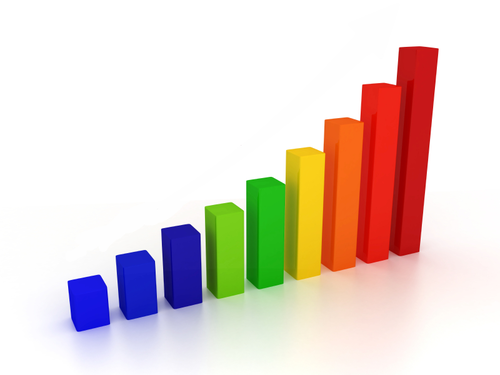
\includegraphics[width=0.5\textwidth]{graph.png}
 % \caption{Графикон}
  %\label{fig:grafikon}
%\end{figure}

% primer jednostavnije matematičke formule
%Ево и један пример математичке формуле: $e^{i\pi} + 1 = 0$. 
% primer referisanja na sliku
%На слици \ref{fig:grafikon} приказан је један графикон.

% primer kompleksnije matematičke formule
%$$
%\int_a^b f(x)\ \mathrm{d}x \ =_{def}\ \lim_{\max{\Delta x_k \rightarrow 0}} \sum_{k=1}^n f(x_k^*)\Delta x_k
%$$

% primer referisanja na poglavlja i strane poglavlja
%Више детаља биће дато у глави \ref{chp:razrada} на страни \pageref{chp:razrada}.

% primer liste
%Можемо правити и набрајања:
%\begin{enumerate}
%\item Анализа 1
%\item Линеарна алгебра
%\item Аналитичка геометрија
%\item Основи програмирања
%\end{enumerate}

%\pangrami

% ------------------------------------------------------------------------------
\chapter{Андроид}
\label{chp:android}
% ------------------------------------------------------------------------------
Андроид је оперативни систем компаније Гугл, отвореног је кода и доступан је под Apache лиценцом  (енг.~{\em Apache Licence}). Apache лиценца је допуштајућа лиценца (енг.~{\em permissive licenses}) и она дозвољава копирање и даље ширење производа без било какве наплате као и дистрибуцију изведеног софтверског производа без обавезе да се к\^{o}д учини јавно доступним \cite{apache,aospapache}.

Андроид се састоји од две велике компоненте: Линукс језгра и пројекта АОСП (енг.~{\em Android Open Source Project}). Дизајниран је пре свега за мобилне уређаје али се данас може користити и у сатовима, сет-топ бокс уређајима, камерама, аутомобилима и другим уређајима. Број активних Андроид уређаја сваким даном се повећава и у моменту писања овог рада, према статистичким подацима Андроид је заступљен на 87,7\% мобилних уређаја у целом свету \cite{marketshare}. На слици \ref{fig:grafikrasta} је приказан график заступљености оперативних система на мобилним уређајима у претходних 8 година.

\begin{figure}[!ht]
\centering
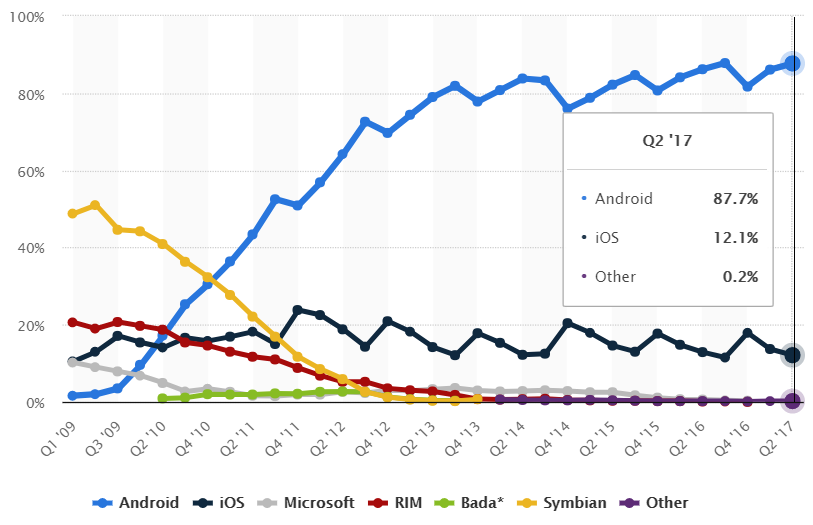
\includegraphics[width=0.9\textwidth]{slike/android87.png}
\caption{График раста популарности Андроида у претходних осам година}
\label{fig:grafikrasta}
\end{figure}

Постоји велика заједница програмера апликација за Андроид који проширују функционалности, уочавају грешке у АОСП-у и развијају велики број апликација које се могу преузети са Гугл продавнице  (енг.~{\em Google Play}). Истраживање спроведено још 2013. године показало је да је Андроид најпопуларнија платформа код 71\% програмера \cite{embeddedandroid}.
\section{Историјат Андроида}
Почеци развоја Андроидa се везују за 2002. годину и компанију Дангер (енг.~{\em Danger}), односно Ендија Рубина (енг.~{\em Andy Rubin}), извршног директора ове компаније \cite{paplukic}. Компанија Дангер је тада имала иновативан производ, мултифункционални телефон са именом Сајдкик (енг.~{\em Sidekick}), о ком је Енди Рубин држао презентацију на којој су, између осталих, присуствовали и оснивачи компаније Гугл Лари Пејџ  (енг.~{\em Larry Page}) и Сергеј Брин  (енг.~{\em Sergey Brin}), за који су се заинтересовали и постали његови корисници. Иако је Сајдкик био иновативан и имао велики потенцијал за даљи развој он ипак није остварио значајан успех а Енди Рубин 2003. године напушта компанију Дангер и оснива компанију Андроид Инц. (енг.~{\em Android Inc.})  која се профилисала ка развоју оперативног система отвореног кода за мобилне уређаје који би се такмичио са већ постојећим Симбијан (енг.~{\em Symbian}) и Виндоус мобајл (енг.~{\em Windows mobile}).\footnote{Енди Рубин, отац Андроида, се поред оперативних система јако интересовао и за роботику.} Гугл 17. августа 2005. године купује Андроид Инц.  за 50 милиона долара.\footnote{Занимљиво је да је, пре него што је Гугл купио Андроид, Енди Рубин покушао продају Андроида Самсунгу који тада није исказао интересовање. } Од 2005. до 2007. Гуглов развојни тим, на челу са Ендијем Рубином, интензивно и у тајности ради на развоју Андроида а тек у новембру 2007. прво саопштење о новом оперативном систему издаје група коју чине компаније чија делатност је мобилна телефонија OXA (енг.~{\em Open Handset Aliance}) попут компанија ХТЦ (енг.~{\em HTC}), Сони (енг.~{\em Sony}), Самсунг (енг.~{\em Samsung}), Ти-мобајл (енг.~{\em T-mobile}), Квалком (енг.~{\em Qualcomm}) i Тексас Инструментс (енг.~{\em Texas Instruments}). Група је основана у сврху развоја отворених стандарда за мобилне уређаје. Име пројекта је AOCП. У септембру 2008. године објављена је прва верзија Андроида и од тада до данас је објављено петнаест верзија Андроида \cite{historyandroid}. Верзије Андроида са датумима објављивања, кодним именом и бројем АПИ-ја (енг.~{\em API- Application Programming Interfaces}) можете видети у табели  \ref{tbl:rezultati}.

\begin{table}
\centering
\begin{tabular}{c>{\centering}p{2cm}cc}
\toprule
\toprule
Кодно име: & Верзија & Датум објављивања & АПИ ниво\\\midrule
N/A & 1.0 & 23. септембар 2008. & 1\\\midrule
N/A & 1.1 & 09. фебруар 2009. & 2\\\midrule
Cupcake & 1.5 & 27. април 2009. & 3\\\midrule
Donut & 1.6 & 15. септембар 2009. & 4\\\midrule
Eclair & 2.0-2.1 & 26. октобар 2009. & 5-7\\\midrule
Froyo & 2.2-2.2.3 & 20. мај 2010. & 8\\\midrule
Gingerbread & 2.3-2.3.7 & 6. децембар 2010. & 9-10\\\midrule
Honeycomb & 3.0-3.2.6 & 22. фебруар 2011. & 11-13\\\midrule
Ice Cream Sendwich & 4.0-4.0.4 & 18. октобар 2011. & 15-15\\\midrule
Jelly Bean & 4.1-4.3.1 & 09. јул 2012. & 16-18\\\midrule
KitKat & 4.4-4.4.4 4.4W-4.4W.2 & 31. октобар 2013. & 19-20\\\midrule
Lolipop & 5.0-5.1.1 & 12. новембар 2014. & 21-22\\\midrule
Marshmallow & 6.0-6.0.1 & 05. октобар 2015. & 23\\\midrule
Nougat & 7.0-7.1 & 22. август 2016. & 24-25\\\midrule
Oreo & 8.0 & 08. август 2017. & 26 \\\midrule
\bottomrule
\end{tabular}
\caption{Верзије Андроида}
\label{tbl:rezultati}
\end{table}

Верзије 1.x и 2.x су намењене телефонима, верзија 3.x таблетима а од верзије 4.x намењене су и мобилним телефонима и таблетима. Кодна имена се дају по абецедном реду при чему је то прво слово неке посластице. 

\section{Развојни модел Андроида и заједница отвореног кода}
Нове верзије Андроида се објављују на приближно шест месеци a новине које долазе са новом верзијом јавности постају познате тек непосредно пред објављивање јер се развој нове верзије Андроида диктира од стране компаније Гугл и практично нико ко није у развојном тиму Гугла не може да утиче на нову верзију Андроида. Разлог за то су Гуглови пословни интереси јер на овај начин Гугл контролише дистрибуцију платформе. Као један од начина да би сваки програмер могао допринети предложеном изменом у развоју нових верзија Андроида настао је CyanogenMod. Он практично представља паралелни развој система али су произвођачи одбили да подрже фирмвер\footnote{Фирмвер је термин који се користи за софтвер смештен на РОМ меморији уређаја и може се заменити флешовањем. Флешовање је краћи назив за поступак који се састоји од прецизно описаног редоследа операција које треба испоштовати за безбедно брисање и поновно писање фирмвера на РОМ меморију.} попут Цианоген мод-а због потенцијалних некомпатибилности незваничног софтвера на уређајима.  Без обзира на Гуглов, помало необичан модел развоја Андроида, чињеница је да је Гугл са Андроидом успео оно што ни један пројекат отвореног кода пре Андроида није успео а то је да створи најраспрострањенији оперативни систем који мобилним уређајима  ставља на располагање моћ и преносивост оперативног система Линукс. Девет година након објављивања прве верзије Андроида он је и даље на узлазној путањи и стално се повећава број и разноврсност уређаја који користе Андроид. 


\section{Архитектура Андроида}
Архитектура Андроид оперативног система је слојевита и састоји се од:
\begin{enumerate}
\item Линукс језгрa (енг.~{\em Kernel layer}) - које се директно ослања на хардвер
\item Радног слоја (енг.~{\em Runtime layer}) :
\begin{enumerate}
\item Скупа извршних библиотека  (енг.~{\em native})
\item Језгра за извршавање Андроид апликација  ({\em Dalvik, ART})
\item Слоја за апстракцију и прилагођавање система
\end{enumerate}

\item Извршног окружења система Андроид (енг.~{\em Android Runtime})
\item Андроид развојног оквира (енг.~{\em Framework layer}) 
\item Апликативног слоја (енг.~{\em Application layer})
\end{enumerate}

\begin{figure}[!ht]
\centering
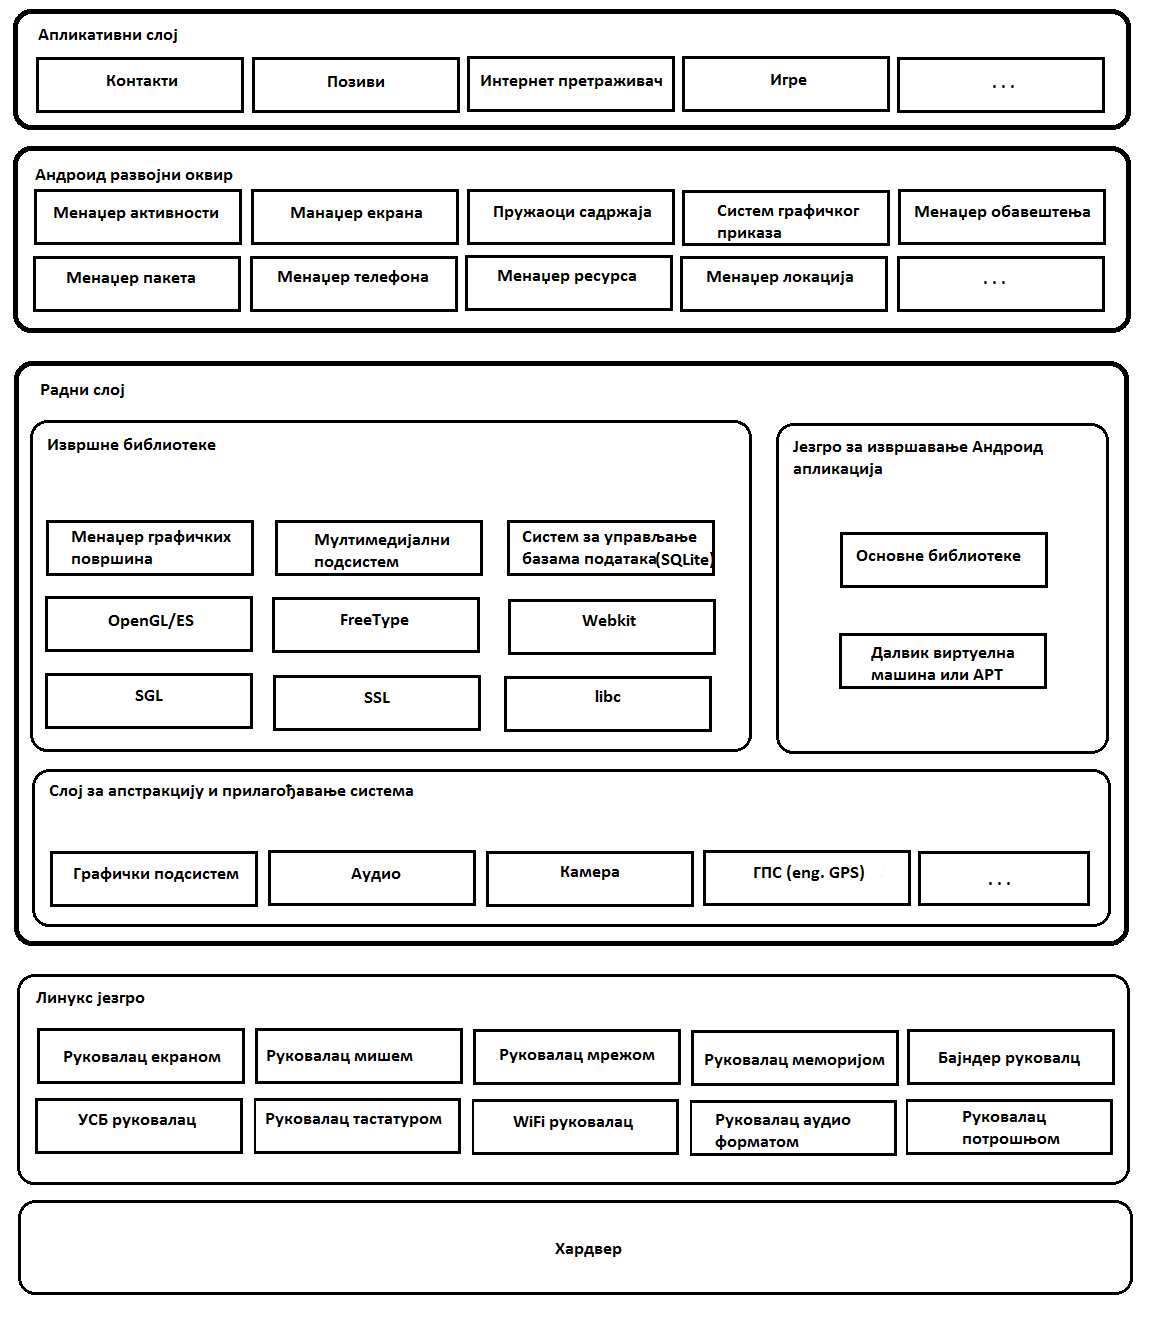
\includegraphics[width=0.9\textwidth]{slike/arhitektiraandroida.png}
\caption{Архитектура Андроид оперативног система}
\label{fig:arhitektura}
\end{figure}
Сликовит приказ архитектуре Андроида можете видети на слици \ref{fig:arhitektura}.

\subsection{Линукс језгро}
Језгро је део система које је само по себи независна целина и не садржи никакве додатне софтверске алате.  Оно пружа основну функционалност оперативног система попут контроле хардверских компоненти и апстракцију свих активних компоненти система у виду процеса, сокета, фајлова итд. Када се систем подиже језгро не мора нужно бити први покренути софтвер али када је једном покренут остаје активан колико и систем. Минимални ресурси потребни за покретање Линукс језгра су:
\begin{enumerate}
\item Процесор брзине 100MHz
\item Рам меморија 2MB
\item Ром меморија 4MB
\end{enumerate}
Минимални хардверски захтеви, робусна и стабилна инфраструктура у сталном развоју и отворен изворни к\^{o}д га чине погодним за мобилне уређаје. Важно је нагласити да Андроид не представља дистрибуцију Линукса већ је само "велика апликација" која се извршава на Линукс језгру. Разлог за то су лиценце и хардверске могућности циљних уређаја. Андроид не поседује неке компоненте које су садржане у Линукс дистрибуцијама попут бибилиотеке glibc која је под лиценцом ГНУ  (енг.~{\em GNU General Public License}). Лиценца ГНУ значи да апликације које користе ову библиотеку морају бити дистрибуиране под истом лиценцом \cite{gnulicence}. Други разлог је величина библиотеке glibc па ни због тога није погодна за мобилне уређаје са мање ресурса. Као алтернатива библиотеци glibc се користи Bionic која је флексибилнија по питању лиценце и омогућава дистрибуцију и под затвореним лиценцама.\\
Линукс језгро је за потребе Андроида проширено апстракцијама попут:

\begin{enumerate}
\item Система за руковање системским временом
\item Binder систем за интерпроцесну комуникацију
\item Ashmem систем за дељење меморије
\item Руковаоцима (енг.~{\em Driver}) за УСБ, тастатуру, жироскоп, вибрацију итд.
\end{enumerate}

\subsection{Радни слој}
Радни слој чине слој за апстракцију, скуп извршних библиотека и Андроид виртуелна машина.

\textbf{Скуп извршних библиотека} садржи значајан број библиотека од којих су неке наменски развијене за Андроид. Оне се директно извршавају на циљном уређају (енг.~{\em native code}) и писане су у програмским језицима C и C++.  Следи неколико примера ових библиотека и њихов кратак опис. \\
\begin{enumerate}
\item Surface Manager - одговоран да сви прозори буду отворени, из потенцијално различитих апликација, у различито време
\item Open GL и SGL - графичке библиотеке за цртање 2Д и 3Д и могу се комбиновати 
\item OkHTTP,  Retrofit, Volley - библиотеке за рад са мрежом
\item WebKit - направљен специјално за мале екране и служи за подршку интернет технологијама
\item SQLite - систем за управљање базама података
\item Media Framework - кодеци за снимање и репродукцију аудио формата, видео формата и слика
\end{enumerate}


\textbf{Слој за апстракцију и прилагођавање система} служи да пружи униформан програмски интерфејс вишим слојевима са циљем да виши програмски слојеви не морају бринути о различитостима циљних платформи. Дакле сврха овог слоја је да омогући независан развој на вишим нивоима а да се промене услед прилагођавања новим платформама праве само у овом слоју.


\textbf{Језгро за извршавање Андроид апликација} у ствари представља виртуелну машину на којој се извршавају Андроид апликације. Постоје два приступа превођењу апликације у машинске инструкције и извршавања на циљној платформи:
\begin{enumerate}
\item Далвик виртуелна машина - прилагођена је мобилним уређајима и оптимизована за рад са ограниченом меморијом и брзином процесора. Бајт-код добијен превођењем програма написаног у програмском језику Јава Далвик виртуелна машина оптимизује и преводи у  ({\em *.dex}) датотеке оптимизиване за извршавање на уређајима са ограниченим ресурсима. Превођење бајт-кода у машински се ради у време извршавања (енг.~{\em JIT Just In Time compilation}). Сваки пут када се покрене нека Андроид апликација прави се нова инстанца Далвик виртуалне машине на којој се апликација извршава.
\item Android RunTime подразумева да се током инсталације апликације бајт к\^{o}д преведе у машински тзв. ELF формат који се чува у меморији  (енг.~{\em AOT-Ahead Of Time compilation}). Последица је да се са оваквим превођењем добија брже извршавање апликације по цену већег утрошка меморије.
\end{enumerate}

\subsection{Андроид развојни оквир}
Представља слој који апликацијама пружа удобан интерфејс у форми Јава класа. У радном слоју се користе програмски језици C/C++ а у апликацијама Јава тако да је задатак овог слоја да преслика позивe функција у Јави на функције у C/C++. То се ради помоћу механизма JNI (енг.~{\em -Java Native Interface}). На овај начин се сва снага и моћ Линукс језгра и библиотека у радном оквиру у виду АПИ-а пружају на коришћење Андроид апликацијама. Свака верзија Андроида има свој АПИ ниво означен одговарајућим бројем (може видети на сајту \url{https://developer.android.com/index.html}) и који представља јединствени идентификатор скупа функционалности дате верзије Андроида.

\subsection{Апликативни слој}
Налази се на врху Андроид софтверског стека и како само име каже чине га апликације. Андроид долази са скупом основних апликација за електронску пошту, СМС поруке, календар, Веб претраживач, контакте и друге апликације. Корисник може преузети или направити сопствену апликацију и инсталирати на уређају. Апликације које долазе са оперативним системом на уређају немају посебан статус и скоро свака се може заменити неком другом која има исту функцију\footnote{Постоје изузеци попут апликације за подешавање система која не може бити замењена.}.

\section{Где је Андроид нашао своје место у овом раду?}
Видели смо да је Андроид оперативни систем са великим могућностима проширивости и примене у разним областима. Такође смо видели да се користи за разноврсне уређаје попут камера, таблета, аутомобила итд. У овом мастер раду искоришћен је Андроид за контролу робота развијеног на Разбери Пај платформи о којој ће бити речи у наредном поглављу. 
Искористићемо мобилни телефон са "Marshmallow" верзијом Андроида и АПИ који ова верзија пружа. За очитавање улаза који задаје корисник искористићемо занимљив сензор,  жироскоп односно акцелерометар, који поседују скоро сви Андроид телефони новијег датума. Акцелерометар је уређај који се може искористити у разне сврхе попут мерења убрзања, пређеног пута, навођење пројектила итд. Рад овог уређаја се заснива на мерењу сила инерције које делују на уређај у току кретања. У средишту кућишта сензора се налази \enquote{велика} и \enquote{тешка} маса, величине делића милиметра, разапета између неколико опруга са ограниченом могућношћу љуљања у простору. Та маса са статичним деловима кућишта формира кондензаторе\footnote{Koндензатор је компонента који може да сачува енергију у облику електричног поља између две електроде раздвојене изолатором.} чији капацитети се мењају у зависности од положаја те масе на коју, током померања уређаја, делују силе инерције. Очитавање вредности сензора се заправо своди на очитавање вредности капацитивности тих кондензатора. Жироскоп служи за мерење промене угла и може се реализовати коришћењем претходно поменутог сензора.

Апликација за навођење робота користи управљачки програм из већ поменутог Линукс језгра како би комуницирала са жироскопом који је хардверски уређај. Адресна магистрала омогућава процесору да приступа уређајима који су повезани на њега и те адресе које су доступне процесору се називају физичке јер представљају адресе стварних физичких компоненти. Физичка адресна мапа представља  стварну локацију сваке компоненте повезане са процесором и њу одређује произвођач уређаја приликом дизајна штампане плоче и повезивања процесора са компонентама. Поред физичког адресног простора постоји и виртуелни у ком се апликација извршава и омогућава да апликације међусобно имају изоловане адресне просторе а језгро има свој физички адресни простор путем кога комуницира са хардверским компонентама. Током извршавања процеса, виртуелне адресе се пресликавају у стварне, физичке адресе. Један пример је оперативна меморија (енг.~{\em RAM-random access memory}). Сваки процес има свој део меморије (виртуални адресни простор) који се захваљујући јединица за управљање меморијом (енг.~{\em MMU-Memory Management Unit}) преводи у физичке адресе на самој хардверској компоненти. Графички приказ пропагације позива од Андроид апликације до самог жироскопа као хардверске компоненте можете видети на слици \ref{fig:propagacija}.


\begin{figure}[!ht]
\centering
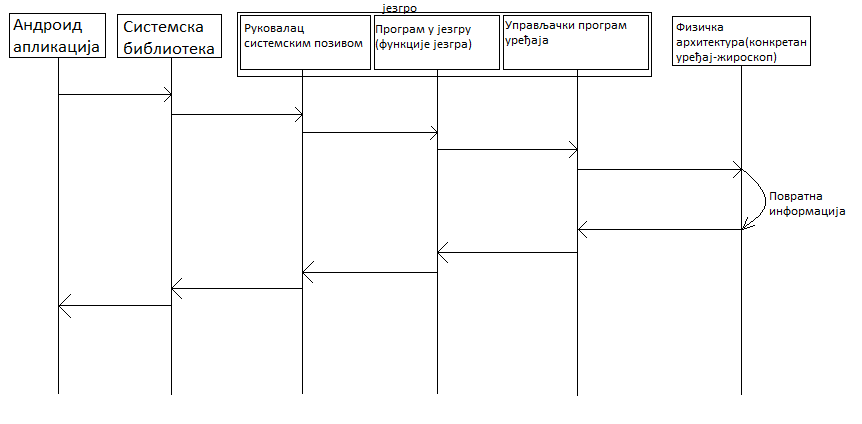
\includegraphics[width=0.9\textwidth]{slike/propagacija_poziva.png}
\caption{Пропагација позива од апликације до очитавања параметара жироскопа}
\label{fig:propagacija}
\end{figure}

Апликација користи одговарајућу системску библиотеку и позива њене функције које врше обраду и системске позиве преко руковаоца системским позивима који даље врши обраде и позива потребне функције језгра. Језгро позива управљачки програм задужен за сензор жироскоп који очитава његов статус и враћа га назад до апликације. На овај начин апликација добија сазнање у ком положају се уређај налази на основу три параметра који се враћају као резултат очитавања. Ти подаци са жироскопа се користе за навођење робота у ком правцу да се креће о ком ће бити више речи у наредним поглављима.

% ------------------------------------------------------------------------------
\chapter{Разбери Пај}
\label{chp:rpi}
% ------------------------------------------------------------------------------
Разбери Пај је рачунар који се може најкраће описати са три речи: мали, моћан и јефтин. Ове три речи су уједно и разлог његове велике популарности и примене у различитим областима интернет ствари (енг.~{\em IoT Internet of Things}), Паметна кућа (енг.~{\em SmartHouse}), едукације и другим.
На тржишту се појавио у фебруару 2012. године, а настао је у истоименој фондацији.

Име Разбери Пај потиче из старе традиције да се компанијама дају имена по воћу. Постоји доста примера попут: енг.~{\em Apricot Computers} - име добијено по кајсији, енг.~{\em Apple} - име добијено по јабуци, енг.~{\em Acorn} - име добијено по једној врсти ораха, енг.~{\em BlackBerry} - име добијено по купини. Разбери Пај је тако добио име по малини, а део Пи потиче од скраћенице \textbf{П}ајтон \textbf{и}нтерпретатор  (енг.~\textbf{P}ython \textbf{i}nterpreter).

\section{Историјат Рaзбери Пај платформе }
Идеја за настанак Разбери Пај платформе се родила почетком прве деценије 21. века на Кембриџу (енг.~{\em University of Cambridge}) због тенденције смањивања броја кандидата заинтересованих за студије Информатике. Још један, можда и важнији, мотив за ову идеју на Кембриџу су видели и у слабом предзнању програмирања оних који се одлуче да студирају. Разлог за то су видели у непостајању платформе довољно занимљиве а опет једноставне и јефтине да заинтригира младе људе и подстакне их на учење и сопствени развој а самим тим и обезбеди боље предзнање будућих студената.

На Кембриџу су до овог закључка дошли кроз анализу претходних генерација које су имале више практичног програмерског знања али и лако програмабилне кућне рачунаре (попут енг.~{\em ZX Spectrum, Commodore 64, Amiga}) које је било потребно програмирати за било какву персонализацију и озбиљнији рад на њима. Генерације са почетка 2000-их су имале лажан привид знања о рачунарским наукама поистовећујући га са корисничким искуством. Због тога се на почетку 21. века свет суочава са недостатком квалификованих ИТ стручњака. Потражња за квалитетним ИТ стручњацима у свету је велика а чак и већа потражња је  вероватна због повећања нашег апетита и очекивања од технологије.

У настојању да се ситуација преокрене Ебен Аптон (енг.~{\em Eben Upton}), тадашњи члан Кембриџ рачунарског одељења, Роб Мулинс (енг.~{\em Rob Mullins}), Џек Ланг (енг.~{\em Jack Lang}), Алан Мајкрофт (енг.~{\em Alan Mycroft}) са Кембриџа, Пит Ломас (енг.~{\em Pete Lomas}) и Дејвид Бребен (енг.~{\em David Braben}) су се удружили 2006. и основали фондацију Разбери Пај \cite{rpibook}. Ова организација је као примарни циљ имала креирање јефтиног, програмабилног рачунара и његово пласирање у што већи број руку. Као резултат заједничког рада, 29. фебруара 2012. је настао Разбери, уређај који нас враћа на рачунарске основе са циљем промоције рачунарства и програмирања код младих. За 6 месеци од момента када се први Разбери појавио продато је 500000 примерака овог рачунара који је поседовао 32-битни Бродкомов\footnote{Бродком је један од највећих произвођача чипова у свету.} чип BCM2835 (енг.~{\em Broadcom}) са АРМ архитектуром (енг.~{\em ARM-Advanced RISC Machines}), брзином од 700MHz и 256MB меморије \cite{rpibook}.

Од тада до данас се појавило више генерација Разбери рачунара а њихове разлике се огледају пре свега у брзини процесора, количини меморије, броја GPIO (енг.~{\em General-purpose Input/Output}) пинова који служе за повезивање и контролисање додатних хардверских компоненти. Прва генерација Разберија је изашла у фебруару 2012. са основним моделом А и моделом Б који је имао више ресурса. Модели А+ и Б+ су се појавили годину дана касније а Разбери 2 модел Б у фебруару 2015. Најновији модел Разбери 3 модел Б који је нама и најзанимњивији, јер је рад урађен управо на овом моделу, појавио се у фебруару 2016. године. У време писања овог рада цена овог рачунара у Србији је око 6000 динара. Хардверске карактеристике овог рачунара можете видети у табели \ref{tbl:rpikonfiguracija}.

\begin{table}
\centering
\caption{Разбери 3 модел Б конфигурација}
\label{tbl:rpikonfiguracija}
\begin{tabular}{ |p{4cm}||p{10cm}|}
	\hline
	Процесор & 1.2GHz 64-bit quad-core ARM Cortex-A53 32kb cache L1 512kb L2\\
	\hline
	Графички процесор & Broadcom VideoCore IV, Opенг.L ES 2.0, 1080p30 h.264/MPEG-4 AVC BluRay quality playback\\
	\hline
	РАМ меморија &  1GB DDR2\\
	\hline
	Складиште података & MicroSD\\
	\hline
	Мрежа & Ethernet RJ45\\
	\hline	
	WiFi & 802.11 b/g/n\\
	\hline
	Bluetooth & 4.1  Low Energy\\
	\hline
	Видео излази & 3.5mm конектор\\
	\hline
	Аудио излази & 3.5mm конектор\\
	\hline
	HDMI & Full HDMI port\\
	\hline
	USB & 4 port\\
	\hline
	GPIO & 40\\
	\hline
	Камера интерфејс (CSI) & да\\
	\hline
	Екран интерфејс (DSI) & да\\
	\hline
	Напајање &  2.5A @ 5V\\
	\hline
	Произведено & UK\\
	\hline
\end{tabular}
\end{table}


\section{Подешавање окружења за рад и инсталација софтвера}
За почетак рада са Разберијем поред самог Разберија је потребно напајање и SD картица. Напајање треба да има прецизно регулисан напон од 5V са једносмерном струјом од 1A до 2,5А. Није могуће користити USB везу са рачунара за напајање Разберија јер оно даје максимално 500mA. Уколико нема додатних компоненти повезаних на Разбери и ако није оптерећен он ће можда радити и на 500mA али ће се с времена на време изненадно ресетовати што може довести до уништавања USB порта на рачунару уколико није заштићен од преоптерећења. Због овога је јако битно да Разбери има посебно напајање од 5V и струјом од 1А. С обзиром да Разбери нема хард диск али има слот за SD картицу потребна је и SD картица. На картици се налази оперативни систем са драјверима и простор за смештање фајлова током рада Разберија. Минимални капацитет картице је 4GB.

За рад са Разберијем је довољна интернет конекција и рачунар са ког се он може контролисати коришћењем SSH\footnote{SSH-Secure Socket Shell је мрежни протокол који обезбеђује сигурну комуникацију са удаљеним рачунаром.} протокола. Монитор, тастатура и миш ипак у многоме могу олакшати посао приликом неких подешавања Разберија.

У случају коришћења монитора најбоље је користити монитор са HDMI улазом јер Разбери има HDMI излаз. Иако је могуће користити и монитор са VGA улазом помоћу HDMI на VGA конвертера потребно је бити пажљив са одабиром конвертера. Конвертер треба да има сопствено напајање јер би у супротном чип за конверзију узимао напајање са Разберија, што би после неког времена направило штету и у најбољем случају прегорела би само заштитна диода а у горем могла би настати штета на самом чипу. Када се користи монитор потребно је прво укључити монитор и сачекати поруку "No HDMI signal" и тек онда покренути Разбери. Што се тиче тастатуре и миша не постоје неки специјални захтеви. Најбоље је одабрати уређаје са каблом и USB конектором како би се избегли потенцијални проблеми са драјверима у случају бежичних уређаја. 

Због заштите самог уређаја приликом повезивања додатних компоненти путем GPIO пинова потребно је нагласити да GPIO пинови, на које се повезују компоненте које примају сигнал од Разберија, као излаз дају 3,3V што је ниво логичке јединице. Они могу безбедно провести струју до 16mA па је због тога потребно бити опрезан приликом повезивања додатних компоненти како не би дошло до прегоревања Разберија. Приликом додавања додатних хардверских компоненти потребно је пажљиво прорачунати коло и ако је потребно додати отпорнике одговарајуће отпорности, везане у редној вези са компонентом, како би се Разбери заштитио од прегоревања. За прорачунавање кола довољно је искористити Омов закон који каже да је струја која пролази кроз проводник између две тачке директно пропорционална напону на истим тачкама тог про\-водника а обрнуто пропорционална његовом електричном отпору $$ I = V/R $$ Након прорачуна кола битно је бити пажљив и на који пин на Разберију повезујете то коло јер немају сви пинови исту сврху. На слици \ref{fig:rpigpioimg} је дат приказ распореда GPIO пинова за Разбери Пај 3 и њихов назив. 

\begin{figure}[!ht]
\centering
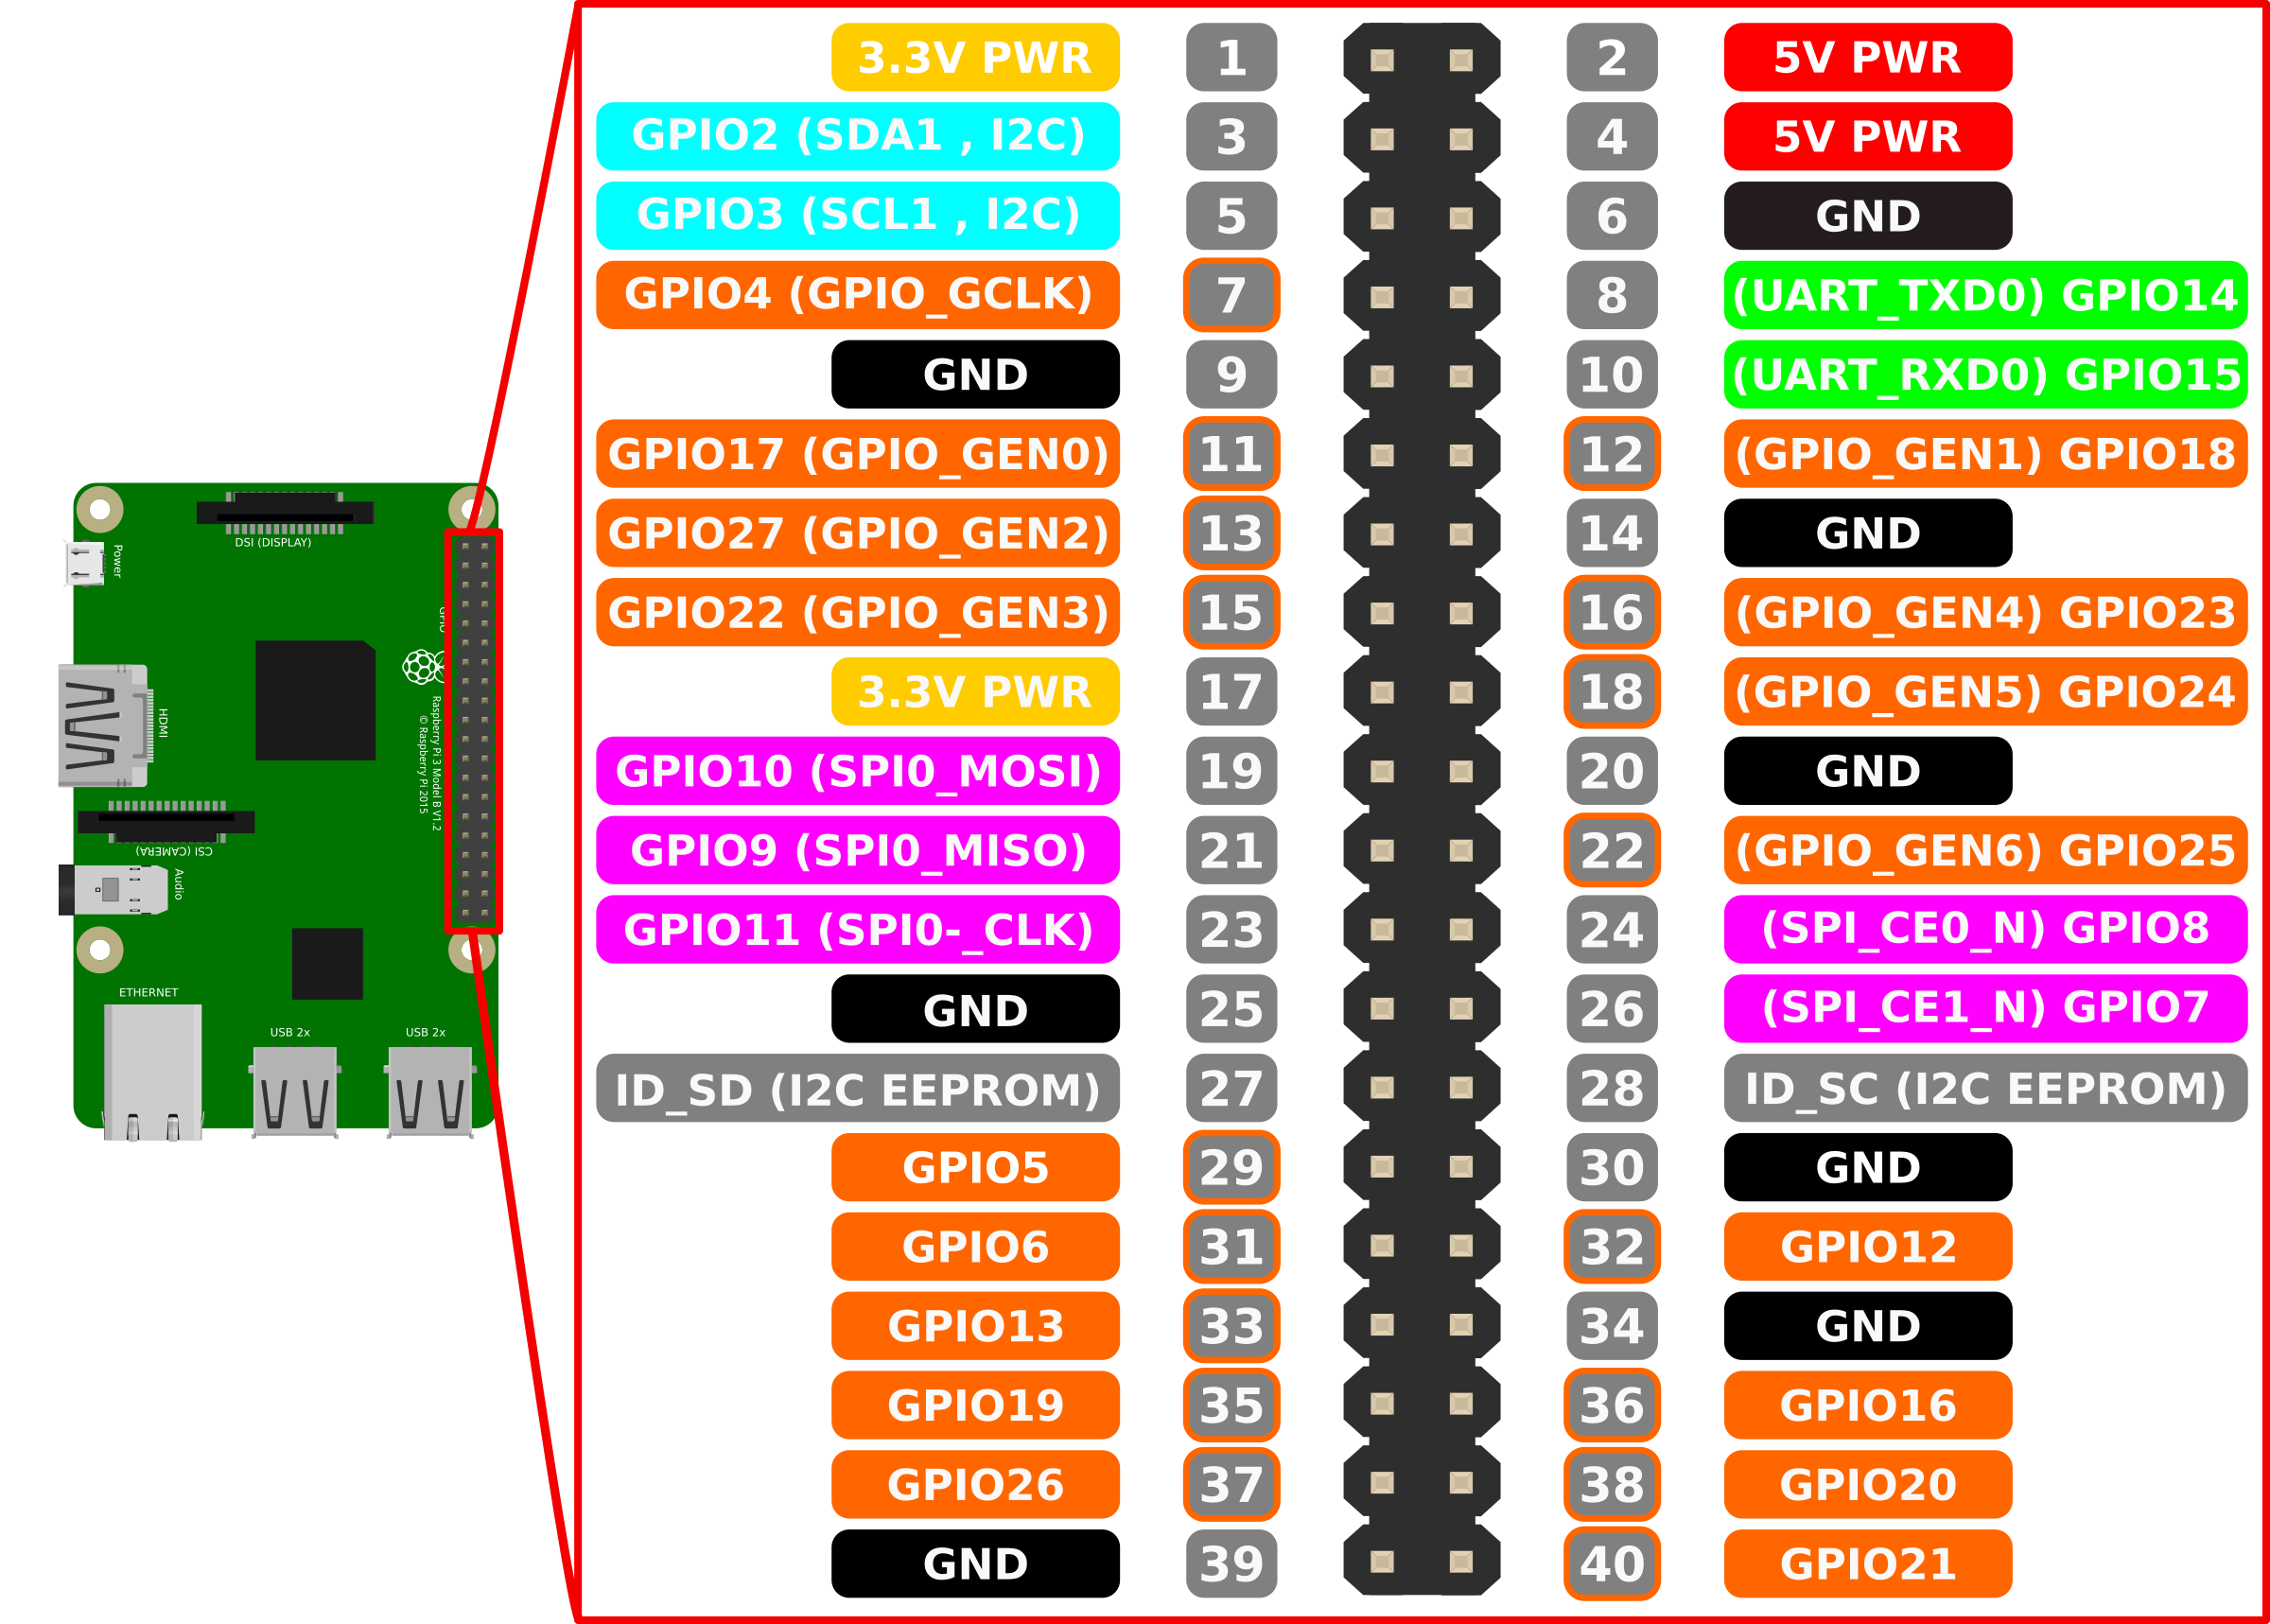
\includegraphics[width=0.9\textwidth]{slike/rpigpio.png}
\caption{Називи и распоред GPIO пинова на Разбери Пај 3}
\label{fig:rpigpioimg}
\end{figure}

\subsection{Инсталација оперативног система}
Разбијан је званични подржани оперативни систем фондације. Може се инсталирати помоћу апликације за инсталацију оперативног система NOOBS или преузимањем слике (енг.~{\em image}) и инсталирањем на картицу. 
За први сусрет корисника са Разберијем препоручује се коришћење NOOBS-а. NOOBS је једноставан софтвер за инсталацију оперативног система који се може преузети са сајта организације. 
Све што је потребно је SD картица, читач SD картице и преузета архива NOOBS-а са сајта\footnote{Уколико немате читач SD картице могуће је са Гугл продавнице (енг.~{\em Google Play Store}) преузети бесплатну апликацију  (енг.~{\em Raspi Card Imager}) на Андроид уређај који поседује SD читач картица и помоћу ове апликације инсталирати NOOBS на картицу.}. Картицу је потребно форматирати и преузету архиву екстрактовати а затим ископирати на SD картицу. Након тога је довољно убацити SD картицу у Разбери и повезати га са монитором, тастатуром, мишем и укључити напајање након чега ће се Разбери бутовати и NOOBS инсталер ће вам понудити опције за инсталацију неколико оперативних система прилагођених за Разбери. Након одабраног жељеног оперативног система (у мастер раду је коришћен Разбијан оперативни систем) и пар кликова добија се SD картица са инсталираним оперативним системом. 

Алтернативни начин, који је и бржи, је преузимањем већ спремљене слике оперативног система са сајта организације. Следи алгоритам за инсталацију оперативног система путем већ спремљене слике оперативног система:
\begin{enumerate}
\item Са сајта организације преузети архивирану слику оперативног система\newline
\url{https://www.raspberrypi.org/downloads/raspbian/} 
\item  Распаковати преузету архиву
\item Преузети и инсталирати Etcher \url{https://etcher.io/} - софтвер за снимање слике оперативног система на SD картицу или USB
\item Покренути Etcher и одабрати распаковану архиву (слику оперативног система) и одабрати SD картицу на коју желите да је сачувате
\item Убацити SD картицу у Разбери и повезати га са монитором, тастатуром, мишем и укључити напајање након чега ће се Разбери бутовати
\end{enumerate}
Када се Разбери бутује нису неопходна никаква додатна подешавања да би почели са радом. Све што је потребно је да се повежете на бежичну везу (енг.~{\em WiFi }) и забава са овим сјајним рачунаром може да почне.

\section{Физичко повезивање Разберија са платформом робота}
Платформа робота коју ће контролисати Разбери је димензија $218mm \times 110mm$. Креће се помоћу три точкића при чему су два погонска и имају своје моторе, по један за сваки од погонских точкова и једног помоћног точка који служи за одржавање равнотеже робота. Платформа је поручена из Кине путем сајта AliExpress и њена цена је око 1300 динара. У овом комплету добијате шасију возила, два мотора, носач за батерије (4 алкалне батерије од по 1,5 V), прекидач за напајање, два точкића са гумама димензија 6,5cm x 2.7cm и један мањи ротирајући точкић. Изглед платформе можете видети на слици \ref{fig:platformarobota}. 

\begin{figure}[!ht]
\centering
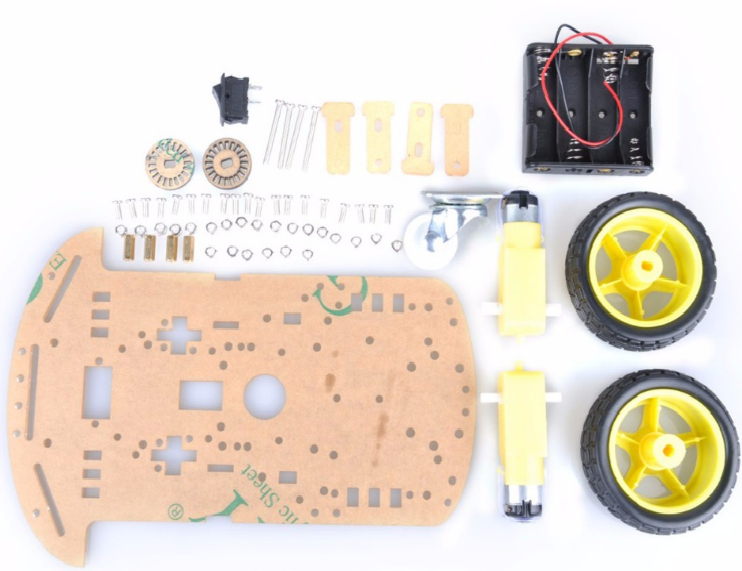
\includegraphics[width=0.9\textwidth]{slike/platforma.png}
\caption{Платформа робота коју контролише Разбери}
\label{fig:platformarobota}
\end{figure}

Мотори су димензија $65mm \times 18.5mm \times 22mm$ и сваки од мотора је директно повезан са својим точком. У питању су ДЦ електромотори који служе да претворе електричну енергију у механичку и углавном раде на принципу електромагнетне индукције. Ови мотори се побуђују једносмерном струјом, углавном се праве за мање снаге и предност им је лакше управљање брзином, моментом и смером обртања. Радни напон им је од 3-12 V (препоручени радни напон 6-8 V) а струја оптерећења 70mA (до максималних 250mA).

Од хардвера је још потребно посебно напајање за Разбери\footnote{Потребно је да Разбери има одвојено напајање како не би долазило до пада напона када се мотори укључе јер би иначе ометали рад Разберија и чак повремено, у случају већег пада напона, довели и до искључивања уређаја.}, развојна плоча за лакше повезивање компоненти, проводници, електрично коло L293D које је заправо мотор контролер и сензор удаљености који ће служити за аутоматско препознавање препреке на путу у режиму аутономног кретања робота ка неком циљу. За напајање је искоришћена преносива батерија за мобилни телефон, капацитета 4400mA, напоном од 5V и струјом од 1,5А. Чип L293D је веома користан чип и он је практично посредник у комуникацији између Разберија и самих мотора. Овај чип може контролисати два мотора независно. Неопходан је како би се избегло да Разберијем директно контролишемо моторе јер мотори могу да повуку већу струју и изазову прегоревање самог Разберија. Овај чип дакле контролише струју и напон за напајање мотора како би Разбери могао неометано да функционише. На овај чип се доводи напајање а онда са њега води на моторе. Излази са Разберијевих GPIO пинова се доводе као логички улази овог кола и од њихових вредности зависи када је који мотор укључен, у ком смеру се окреће и којом брзином односно када коло проводи или не проводи струју и на тај начин напаја моторе. Назив и кратак опис сваког пина за коло L293D се налази у табели \ref{tbl:l293dconfig}.


\begin{figure}[!ht]
\centering
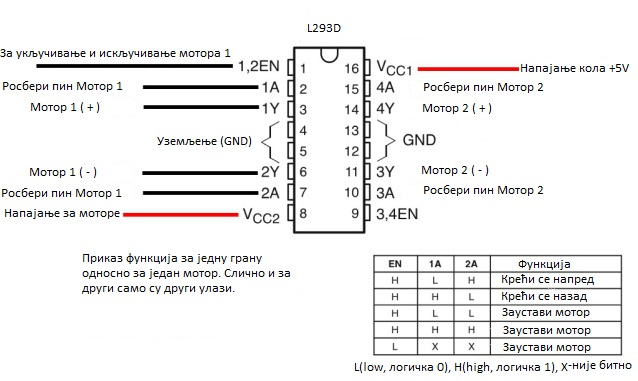
\includegraphics[width=0.9\textwidth]{slike/shemal293d.jpg}
\caption{Мотор контролер L293D}
\label{fig:l293d}
\end{figure}



\begin{table}
\centering
\caption{Називи и опис функција пинова на чипу L293D}
\label{tbl:l293dconfig}
\begin{tabular}{ |p{1cm}||p{10cm}|p{2cm}|}
	\hline
	Пин & Опис његове функције & Назив\\
	\hline
	1 & Укључивање контроле над мотором 1 (Мотор реагује на сигнале за смер кретања са пинова 1  2) & Enable 1,2 \\
	\hline
	2 & Улаз 1 за мотор 1  & Input1 \\
	\hline
	3 & Излаз 1 за мотор 1 & Output1\\
	\hline
	4 & Уземљење (0V) & Ground\\
	\hline
	5 & Уземљење (0V) & Ground\\
	\hline
	6 & Излаз 2 за мотор 1 & Output2\\
	\hline
	7 & Улаз 2 за мотор 1  & Input2 \\
	\hline
	8 & Напон напајања за моторе 9-12V (до максималних 36V) & Vcc2 \\
	\hline
	9 & Укључивање контроле над мотором 2 (Мотор реагује на сигнале за смер кретања са пинова 3 и 4) & Enable 3,4 \\
	\hline
	10 & Улаз 1 за мотор 2 & Input3\\
	\hline
	11 & Изалаз 1 за мотор 2 & Output3\\
	\hline
	12 & Уземљење (0V) & Ground \\
	\hline
	13 & Уземљење (0V)& Ground \\
	\hline
	14 & Излаз 2 за мотор 2 & Output4\\
	\hline
	15 &  Улаз 2 за мотор 2 & Input4 \\
	\hline
	16 & Напон напајања за чип 5V (до максималних 36V) & Vcc1\\
	\hline
\end{tabular}
\end{table}


Као сензор удаљености искоришћено је коло HC-SR04 за прецизно мерење растојања користећи ултразвучно мерење. Димензије кола су $16mm \times 50mm$ и може да мери удаљеност на раздаљини од 2cm до 450cm са малом грешком од 0.3cm. За што прецизније мерење битно је сензор поставити тако да сензор гледа хоризонтално са углом у односу на хоризонталу не већим од 15 степени. Радни напон је 5V а радна струја 15mA. Коло има 4 пина. Један служи за напајање, један за уземљење, један је за окидање (слање ултразвучног сигнала) и један пин је ехо (повратна информација). Сензор ради тако што емитује ултразвучне импулсе\footnote{Звучни импулси фреквенције изнад горње границе чујности за нормално људско ухо, преко 20kHz.}  и мери време од тог тренутка до тренутка када добије повратну информацију односно до тренутка када сензор прими импулсe који су се одбили од потенцијално постојеће препреке. Формула за рачунање растојања до препреке (уколико постоји) је: $$ D = V*t $$
При чему је D - растојање, V - брзина ултразвучног сигнала кроз ваздух и t- протекло време од слања ултразвучног сигнала са сензора до детектовања његовог еха на сензору.
Изглед овог кола (сензора) и илустрацију начина рада можете видети на слици \ref{fig:ultrasonicsensor}. 

\begin{figure}[!ht]
\centering
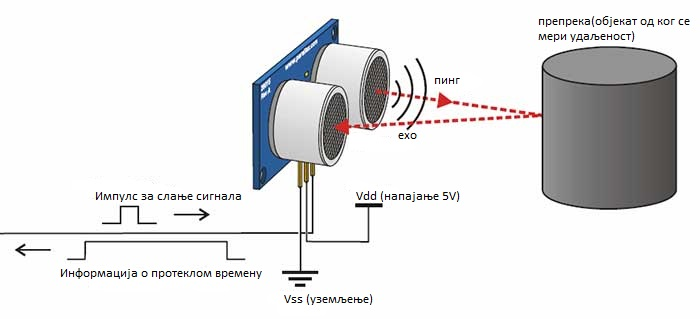
\includegraphics[width=0.9\textwidth]{slike/UltrasonicSensors.jpg}
\caption{Принцип рада и изглед сензора удаљености }
\label{fig:ultrasonicsensor}
\end{figure}

Све горе описане компоненте (Разбери, развојну платформу робота, моторе, сензоре, чип L293D, батерије) је потребно повезати у једну целину која ће чинити робота. Шему за повезивање ових компоненти можете видети на слици \ref{fig:mainshema}.

На робота је постављено три сензора удаљености тако да је један постављен у правцу кретања робота и по један лево и десно под угловима од -90 и +90 степени у односу на правац кретања робота. Користи се више сензора због бољег решавања колизија у режиму аутономног кретања робота.

\begin{figure}[!ht]
\centering
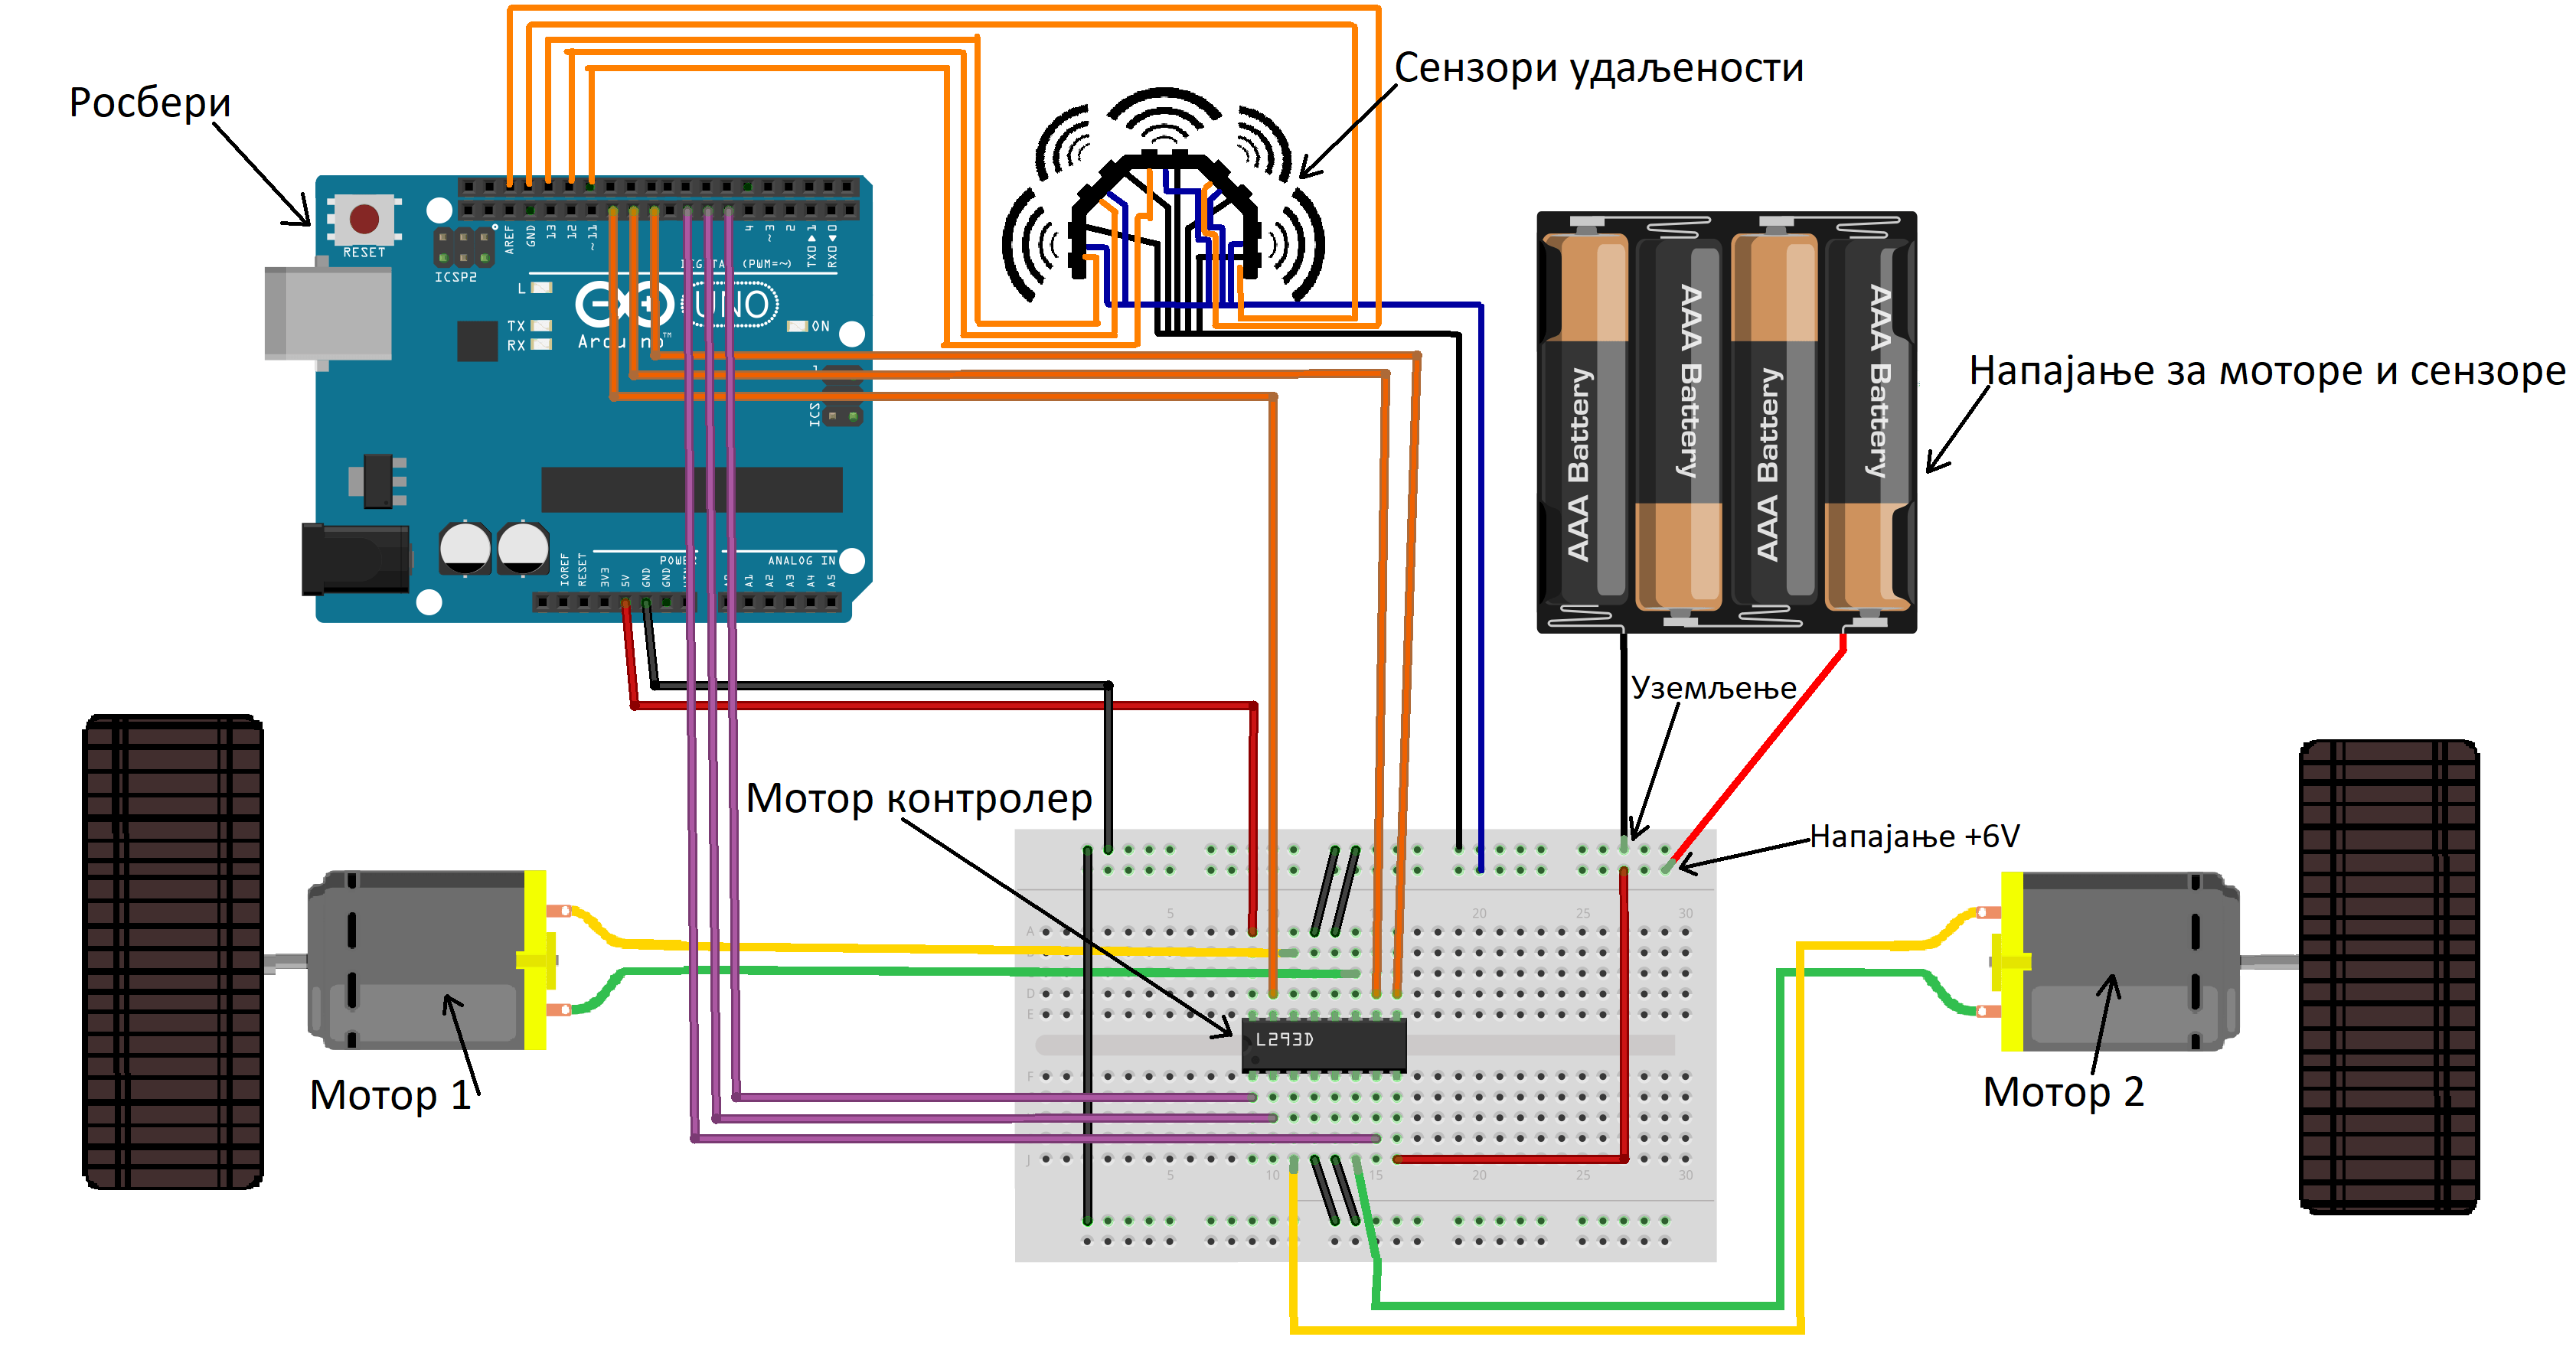
\includegraphics[width=0.9\textwidth]{slike/shema.png}
\caption{Шема за повезивање Разберија са платформом и сензорима }
\label{fig:mainshema}
\end{figure}

Шема илуструје оно што је до сада објашњено и дат је један од могућих начина за повезивање Разберија са платформом робота и сензорима онако како је то урађено на роботу. Сада када је потребан хардвер повезан у функционалну целину долази ред на софтверски део и имплементацију која ће се састојати из три битне целине:
\begin{itemize}
\item Андроид апликације за телефон - служи као кориснички интерфејс за руковање роботом
\item Пајтон  (енг.~{\em Python}) апликације за Разбери - служи да управља роботом односно да прима наредбе од корисника (Андроид апликације) и да их преводи у одговарајуће реакције хардвера
\item Имплементација алгоритма за аутономно кретање - служи да робота учини ,,интелигентним''
\end{itemize}

У наредна два поглавља је дат опис алгоритма, његов начин рада и опис имплементације а након тога и комплетан систем са апликацијама и алгоритмом.

% ------------------------------------------------------------------------------
\chapter{Алгоритам заобилажења препреке}
\label{chp:algoritam}
% ------------------------------------------------------------------------------
Поред тога што се робот може наводити ручно, помоћу Андроид апликације, лепота и сврха постојања роботике се огледа управо у томе да робот може сам да обавља неки задатак без помоћи човека. Савремени роботи решавају реалне проблеме у динамичном и отвореном окружењу. Због тога се појављују нови изазови у областима алгоритама контроле робота и планирања покрета. Ови изазови се јављају услед повећане потребе за аутономијом и флексибилношћу робота. Jедан од основних задатака роботике је ,,научити'' робота да се самостално креће без асистирања човека. У овом поглављу биће описан БАГ (енг.~{\em BUG}) алгоритам који се бави проблемом планирања путање кретања робота. Након тога биће речи о томе како је овај алгоритам прилагођен за потребе овог рада.

БАГ алгоритам служи за планирање путање робота од стартне до циљне тачке у дводимензионалном простору без информација о изгледу мапе терена\footnote{Под мапом терена се мисли на слику или поглед из ваздуха на област кроз коју се робот креће и чијом анализом се могу применити неки други и ефикаснији алгоритми за проналажење оптималне путање.} и могућим препрекама. С обзиром да се роботи не морају користити искључиво у фабрикама, кућама или негде другде где постоји устаљена мапа терена, овај проблем кретања робота у ,,непознато'' je утолико занимљивији и шире применљив. БАГ алгоритам је један од првих алгоритама  базираних на контактним сензорима или сензорима дистанце и гарантује проналажење решења у коначном броју корака уколико је циљ достижан. 

Најбитније три верзије овог алгоритма су: БАГ1, БАГ2 и тангентни алгоритам БАГ (енг.~{\em Tangent BUG algorithm})\footnote{Постоји још неколико верзија које користе основне идеје БАГ алгоритма са додатком разних хеуристика за проналажење што бољег решења у задатим условима.}. БАГ1 и БАГ2 алгоритми претпостављају поседовање контактних сензора док тангентни алгоритам БАГ претпоставља поседовање сензора који могу прецизно мерити дистанцу до неког објекта у свих 360 степени. Без обзира на врсту сензора, све три верзије карактеришу двe особине: кретање ка циљу правом линијом и заобилажење препреке праћењем њене контуре \cite{principlesofrobotmotion}. 

Постојe и други напреднији алгоритми за овај проблем али сваки од тих напреднијих алгоритама почива на претпоставкама попут поседовања:
\begin{itemize}
\item Снажних сензора (домет сензора је велики)
\item Доста рачунарске снаге за сложена израчунавања
\item Доста меморије за чување мапе
\item Прецизних GPRS уређаја
\item Слике из ваздуха (са висине која може да посматра већи простор)
\end{itemize}

У наставку рада ће бити демонстрирано да није неопходна скупа опрема и снажни рачунари за аутономно кретање робота. Довољан је један јефтин сензор дистанце и Разбери  на ком ће се извршавати БАГ алгоритам да би се овај проблем решио.

\section{Како раде БАГ1 и БАГ2 алгоритми?}
За самостално кретање робота у овом раду су искоршћене основне идеје БАГ1 и БАГ2 алгоритма. Прецизније, БАГ2 алгоритам је модификација БАГ1 алгоритма и он је прилагођен за потребе овог рада. Пре самог описа алгоритама битно је нагласити да су они засновани на одређеним претпоставкама. Неке од њих у реалним применама могу бити проблематичне. Претпоставке које се користе у алгоритму су:
\begin{itemize}
\item Робот је тачка са савршеним позиционирањем (кретање односно положај робота се може пратити савршено прецизно)
\item Робот може открити препреку уколико је додирне
\item Робот може прецизно мерити растојање између било које две тачке $d(x,y)$
\item Простор $W$ у ком се робот креће је ограничен
\end{itemize}

Тачку са које робот креће означићемо са $q_{start}$ а тачку која представља циљ, који робот треба да достигне, означићемо са $q_{goal}$. У алгоритму се користе појмови тачке поготка, тачке напуштања и $m$-линије. Тачка поготка је тачка у којој је детектована колизија са другим објектом током кретања робота ка циљу. То је тачка у којој се робот сударио са препреком и означава се са $q_i^H$. Индекс $i$ означава редни број препреке са којом је робот дошао у колизију током кретања а ознаке $H$  (енг.~{\em \textbf{H}it}) и $L$ (енг.~{\em \textbf{L}eave}) говоре о томе да ли је тачка са индексом $i$ тачка поготка или тачка напуштања. Тачка напуштања је тачка у којој се робот одваја од контуре препреке након њеног заобилажења и означава се са $q_i^L$. У алгоритму БАГ1 $m$-линија је линија која спаја тачке $q_i^L$ и $q_{goal}$. Она се користи током праволинијског кретања робота ка циљу.

На почетку алгоритма се узима да је тачка $q_0^L = q_{start}$ и бројач препрека $i=0$. Робот одређује $m$-линију од тачке  $q_0^L$ до $q_{goal}$ и започиње кретање по њој ка циљу. Уколико дође до циља алгоритам се завршава јер је решење пронађено. Уколико је током кретања $m$-линијом дошло до колизије (робот је детектовао препреку на свом путу) робот увећава бројач препрека $i=i+1$ и тачку у којој је дошло до колизије означава са $q_i^H$ и памти њене координате. Затим кружи око препреке, пратећи њене контуре, све док се не врати у тачку $q_i^H$. Тада има довољно знања о препреци да може да одреди тачку на контури препреке која је најближа циљу (тачки $q_{goal}$). Та тачка је тачка напуштања за $i$-ту препреку и биће означена са $q_i^L$. Робот се креће до тачке $q_i^L$ и ажурира $m$-линију и наставља кретање. Уколико новодобијена линија пресеца тренутну препреку закључак је да не постоји пут до циља односно робот се налази унутар затворене препреке \cite{principlesofrobotmotion}. Илустрaцију начинa рада алгоритма БАГ1 можете видети на слици \ref{fig:bug1}.

\begin{figure}[!ht]
\centering
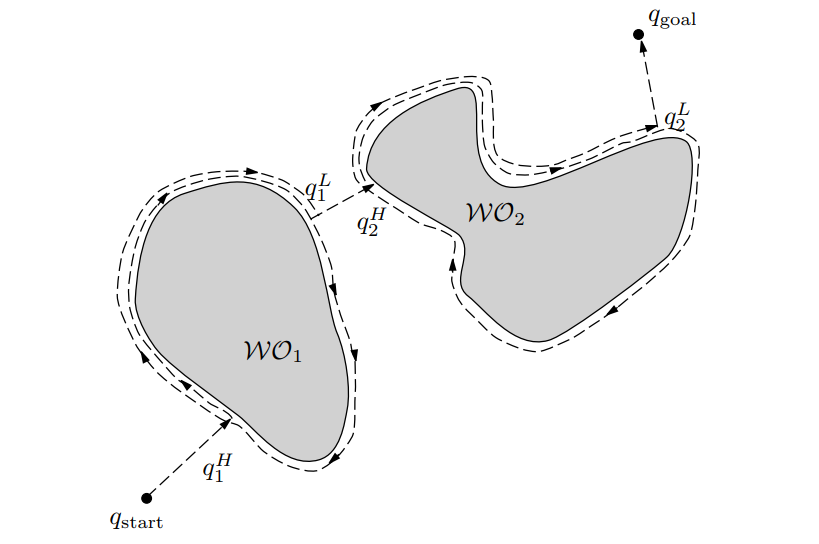
\includegraphics[width=0.9\textwidth]{slike/bug1.png}
\caption{Начин рада алгоритма БАГ1}
\label{fig:bug1}
\end{figure}

БАГ2 алгоритам представља модификацију алгоритма БАГ1. Основне разлике су то што се $m$-линија код БАГ2 алгоритма не мења током извршавања алгоритма. Она је фиксна и повезује тачке $q_{start}$ и $q_{goal}$. Још једна разлика је у томе што када робот наиђе на препреку (тачка поготка) не обилази целу њену контуру. У тачки поготка се случајним избором одлучује са које стране ће обилазити препреку и започиње праћење контуре препреке све док се поново не нађе на $m$-линији (тачка напуштања). У тачки напуштања се одваја од препреке и наставља кретање ка цињу по $m$-линији. Илустрација начина рада алгоритма БАГ2 може се видети на слици \ref{fig:bug2}.
\begin{figure}[!ht]
\centering
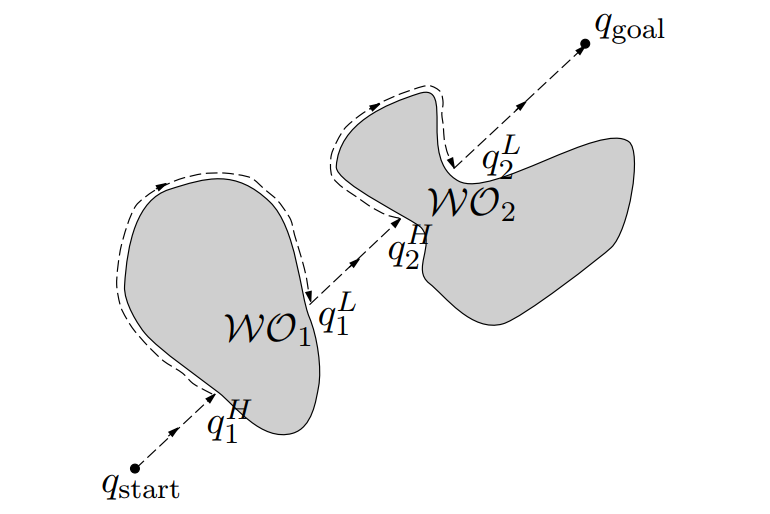
\includegraphics[width=0.9\textwidth]{slike/bug2.png}
\caption{Начин рада алгоритма БАГ2}
\label{fig:bug2}
\end{figure}
Ако се робот два пута нађе у истој тачки поготка $q_i^H$ тада закључује да не постоји пут до циља јер се налази у затвореној препреци (нема излаз из затворене препреке). Овај случај можете видети на слици \ref{fig:bug2f}.

\begin{figure}[!ht]
\centering
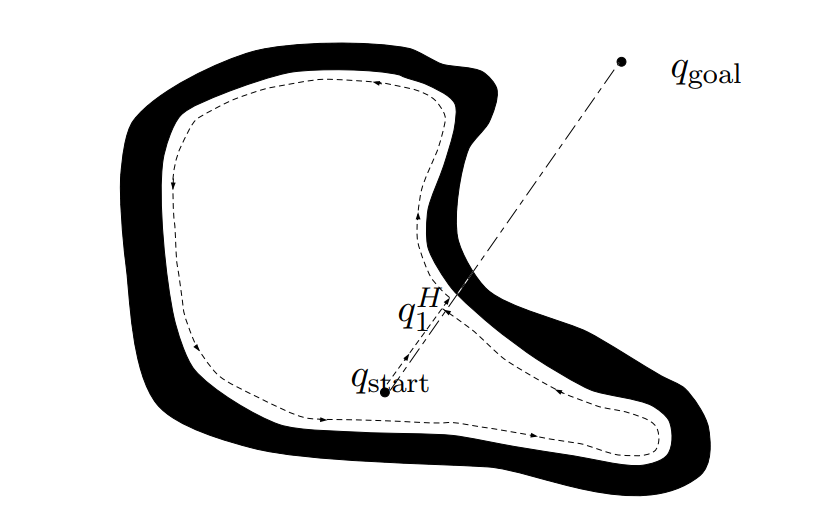
\includegraphics[width=0.9\textwidth]{slike/bug2f.png}
\caption{Детекција случаја када не постоји пут до циља}
\label{fig:bug2f}
\end{figure}

Ова два алгоритма илуструју два основна приступа за проблеме претраживања. Алгоритам БАГ1 проналази оптималну тачку напуштања за сваку препреку на коју наиђе али по цену да ради исцрпну претрагу. Алгоритам БАГ2 користи похлепни приступ јер гледа само локалну добит односно бира прву опцију која му у том тренутку обећава проналажење решења.

\section{Како робот користи БАГ алгоритам?}
Током навођења робота помоћу Андрид апликације могу се десити колизије. Робот је ,,паметан'' и неће дозволити човеку да га води у ,,опасност''. Када детектује препреку на путу којим га води човек робот се сам зауставља. Он нуди човеку могућност да га човек води другачијим путем или да му препусти да се сам снађе и превазиђе проблем. Уколико човек препусти контролу роботу након обилажења препреке, уколико је то могуће, робот враћа контролу човеку. Имплементиран алгоритам се у великој мери ослања на алгоритам  БАГ2 јер користи његову идеју приликом заобилажења препреке. Дакле, не ради исцрпну претрагу као БАГ1 већ користи похлепни приступ па се може рећи да је сличнији БАГ2 алгоритму. Зависно од примене робота и један и други алгоритам се могу применити. У овом раду се не проналази оптимално решење већ оно које ће у реалном раду робота дати брже решење односно оно које ће робота брже довести до циља. Коришћење БАГ1 алгоритма има смисла када робот треба да научи неки пут и да га после поново користи али када је основни циљ стизање до неке тачке у ,,непознатом'' оправданије је користити БАГ2 алгоритам.

Дакле, у основи алгоритма који користи робот за аутономно кретање се налази БАГ2 алгоритам. Овом алгоритму је, за разлику од БАГ2 који користи само контактни сензор, на располагање дат сензор дистанце или тачније неколико сензора дистанце. Ови сензори могу да детектују препреку на неколико метара. Захваљујући њима робот, у тренутку када му се препусти контрола да сам заобиђе препреку, не бира баш на потпуно случајан начин страну са које ће заобићи препреку већ је мало анализира помоћу сензора. Тачније робот може да ,,погледа'' лево и десно пре него крене и да процени где му је отворенији пут. Више сензора је постављено под различитим угловима у односу на правац кретања из разлога да робот не мора да физички прави заокрете како би направио ово процену. У наставку следи опис како је алгоритам практично имплементиран.

За рад алгоритма је потребно успоставити неки координатни систем у ком се робот налази. Правац у ком је усмерен робот одређује $y$ осу координатног система а нормала на тај правац, кроз тачку у којој се налази робот, одређује $x$ осу. Смер у ком робот ,,гледа'' одређује позитивни део $y$ осе, иза робота је негативни део $y$ осе, десно позитивни део $x$ осе а лево негативан део $x$ осе. Овај координатни систем се успоставља на почетку рада алгоритма и до краја се не мења али ће робот током кретања мењати своје координате у овом систему.

Робот током кретања, помоћу сензора постављеног са предње стране, непрестано проверава да ли му се на путу налази препрека. Када детектује да му је препрека на путу то јавља човеку (апликацији за навођење) и нуди опцију да га води другим путем или да му препусти да заобиђе препреку и да му након тога врати контролу. Када му човек преда контролу он рачуна $m$ - линију\footnote{$m$ - линија ће заправо бити $y$ оса координатног система који се поставља у том тренутку.} и помоћу сензора дистанце постављених под угловима од -90, -45, +45 и +90 степени, проверава да ли му је у неком смеру слободан пут. Ако јесте, критеријуми за одабир новог правца кретања $v$ робота су:
\begin{itemize}
\item што мањи угао између $m$ - линије и правца $v$
\item непостојање или што веће растојање до нове колизије у правцу $v$ у домету сензора дистанце
\item оба сензора дистанце (парови (-90,-45) i (+45,+90)) са стране робота на којој се налази правац $v$  сигнализирају слободан пут
\end{itemize}

Уколико није добио ни један позитиван одговор, робот на случајан начин бира страну и врши постепен заокрет у одабрану страну радећи исте провере све док не добије позитиван одговор са неког од сензора. На основу добијеног позитивног одговора, или више њих, и положаја сензора са кога је добијен тај одговор робот бира најбољи по горе наведеним критеријумима.

Када је нови правац кретања робота одабран потребно је сачувати информацију о томе да ли кретањем у одабраном правцу $v$ робот иде лево или десно у односу на $m$ - линију тј да ли обилажење препреке иде са леве или са десне стране. Ова информација је битна за праћење контуре препреке.

Робот започиње кретање по одабраном правцу непрестано проверавајући сензор са предње стране и два сензора десно ако препреку обилази са леве стране или два сензора лево ако препреку обилази са десне стране. 

\begin{figure}[!ht]
\centering
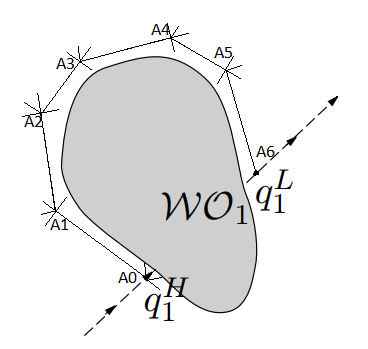
\includegraphics[width=7cm, height=6cm]{slike/adapt_bug.png}
\caption{Начин рада БАГ2 алгоритма на роботу}
\label{fig:bugadapt}
\end{figure}

За сензоре са бочне стране робота (под угловима од 45 и 90 степени) у дањем тексту користи се ознака $S$. Робот се креће у одабраном правцу све док неки од сензора из $S$ не пријави слободан пут и тада робот поново мења правац. Робот мери пређени пут од претходне тачке промене правца $A_{i}$ и бележи нове координате у којој је променио правац. На тај начин се прати контура препреке а обилажење је готово када се робот поново нађе на $m$ линији односно када му $y$ координата поново постане 0. Илустрација начина на који робот заобилази препреку може се видети на слици  \ref{fig:bugadapt}.

Када је робот обишао препреку наставља да се креће напред све док човек поново не преуме контролу.


% ------------------------------------------------------------------------------
\chapter{Апликација RPiDroid}
\label{chp:aplikacija}
% ------------------------------------------------------------------------------
Софтверско решење које се користи за навођење и контролу робота се заснива на клијент-сервер архитектури и састоји се од:
\begin{itemize}
\item Андроид апликације
\item Пајтон сервера
\end{itemize}

Клијентску страну представља Андроид апликација која се извршава на мобилном телефону или таблету. Служи да улазне информације добијене од корисника проследи Пајтон серверу и да повратну информацију од робота прикаже кориснику.

Серверску страну представња Пајтон сервер на Разберију и састоји се од три битна модула:
\begin{itemize}
\item Модул за комуникацију са апликацијом
\item Модул за контролу платформе робота
\item Модул за аутономно кретање
\end{itemize}

Следи детаљнији опис сваког дела софтвера.

\section{Имплементација Андроид апликације}
Андроид апликације могу бити писане у програмским језицима Котлин (енг.~{\em Kotlin}), Јава (енг.~{\em Java}) или C++. За навођење робота је направљена Андроид апликација коришћењем програмског језика Јава и развојног окружења SDK (енг.~{\em Software Development Kit}) за Андроид. Апликације направљене на овај начин се називају и нативне (енг.~{\em native}) апликације и програмерима дају потпуну слободу и приступ могућностима и сензорима уређаја. 

Основни градивни елементи сваке Андроид апликације су следеће компоненте:
\begin{itemize}
\item Активности  (енг.~{\em Activity})
\item Сервиси (енг.~{\em Services})
\item Пружаоци садржаја (енг.~{\em Content providers})
\item Пријемници емитованих обавештења (енг.~{\em Broadcast receivers})
\end{itemize}

Активности су компоненте чија је сврха приказивање корисничког интерфејса и интеракција са корисником. Већина апликација се састоји из једне или више активности чији интерфејс се обично дели у фрагменте који представљају модуларне делове активности. Апликација не мора нужно имати активности уколико је реч о апликацији која ради у позадини и није видљива кориснику. Апликације које користе активности их имплементирају као поткласе класе ,,Activity''.

Сервиси су компоненте које немају кориснички интерфејс и служе за обављање послова у позадини апликације. Сервиси имају свој АПИ и пружају услуге активностима или другим сервисима. Користе се углавном за дуготрајне операције попут комуникације преко мреже или за одржавања апликације у стању извршавања иако корисник можда тренутно користи неку другу апликацију. У апликацијама се имплементирају као поткласа класе ,,Services''.

Пружалац садржаја је компонента која управља скупом података апликације који се чувају у фајл систему, бази података, на вебу или било којој другој локацији којој апликација има приступ. Друге апликације могу да читају и мењају те податке уколико им то пружалац садржаја дозволи. У апликацијама се имплементира као поткласа класе ,,ContentProvider'' и мора да имплементира скуп АПИ-а који ће друге апликације подразумевати.

Пријемник емитованих обавештења је компонента апликације која омогућава да се укључи ,,хватање'' догађаја (енг.~{\em event}) на систему. Другим речима, ова компонента апликације каже оперативном систему да је обавести када се одређени догађај појави. Апликација не мора бити у стању извршавања да би одговорила на догађај већ се њено покретање може иницирати догађајем. Имплементира се као поткласа класе ,,BroadcastReceiver''.

Још једна неизоставна ствар коју свака Андроид апликација мора имати је фајл AndroidManifest.xml. Све компоненте од којих се апликација састоји морају бити наведене у овом фајлу. Такође је потребно навести и дозволе које су потребне апликацији за исправан рад. То може бити приступ камери, именику, жироскопу или било шта друго што постоји на уређају а није подразумевани ресурс апликације. Обавезно је и навођење минималног и циљаног АПИ-а односно верзије Андроида за коју је апликација написана. 

Апликација за навођење састоји се од две активности и једног сервиса. Због јаснијег описа прво ће бити приказан и описан кориснички интерфејс и случајеви употребе па тек онда технички детаљи имплементације. 

Прва активност служи за унос ИП адресе робота и успостављање везе са роботом. Изглед корисничког интерфејса ове активности можете видети на слици \ref{fig:activity1}.

\begin{figure}[!ht]
\centering
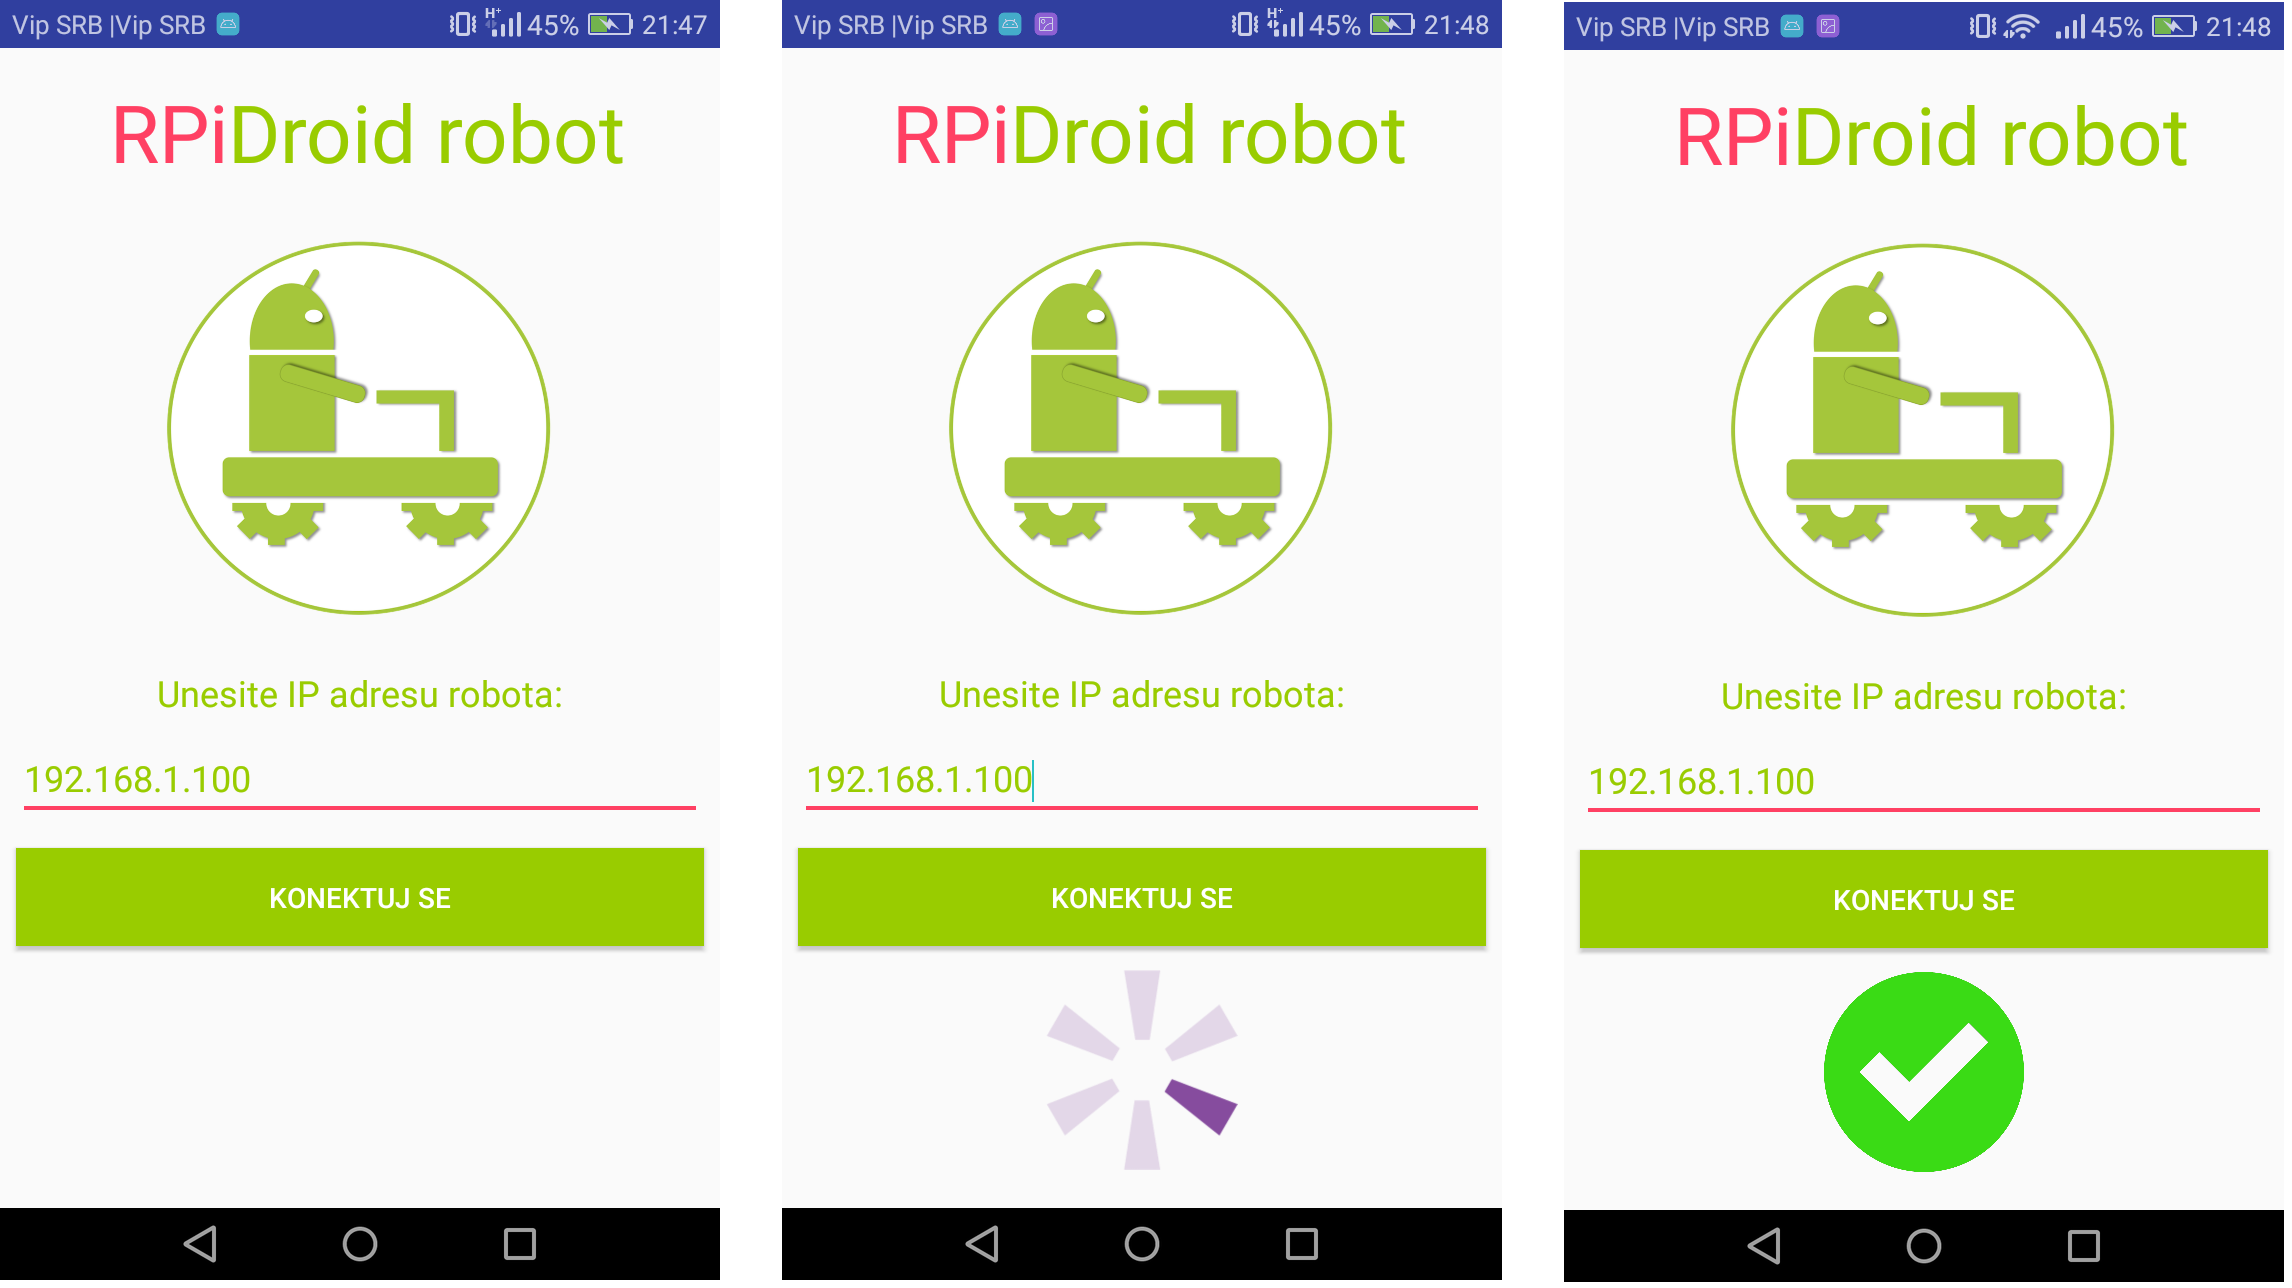
\includegraphics[width=0.9\textwidth]{slike/povezivanje.png}
\caption{Успостављање везе између апликације за навођење и робота}
\label{fig:activity1}
\end{figure}

Када робот одговори да је спреман да прихвата наредбе, веза је успостављeна и покреће се друга активност која служи као интерфејс за управљање роботом. Она је централна компонента у апликацији. Из ње се очитава сензор жироскопа коришћењем системских сервиса намењених за то и врши комуникација са роботом коришћењем сервиса направљеног за потребе апликације. Ова активност има неколико ствари које приказује. Једна од информација је стања сензора жироскопа у виду стрелица које показују на коју страну је нагнут уређај на ком се извршава апликација. Ове стрелице означавају правац у ком наводимо робота да се креће. У овој активности се налазе и два контролна дугмета. Једно служи за укључивање аутономног режима кретања а друго је команда којом се прекида сваки посао и робот се зауставља. Аутономни режим подразумева кретање робота право напред а уколико наиђе на препреку сам треба да се снађе и заобиђе је. Из аутономног режима се излази притиском на дугме за заустављање. Изглед корисничког интерфејса активности за навођење робота можете видети на слици \ref{fig:uiactivity2}.

\begin{figure}[!ht]
\centering
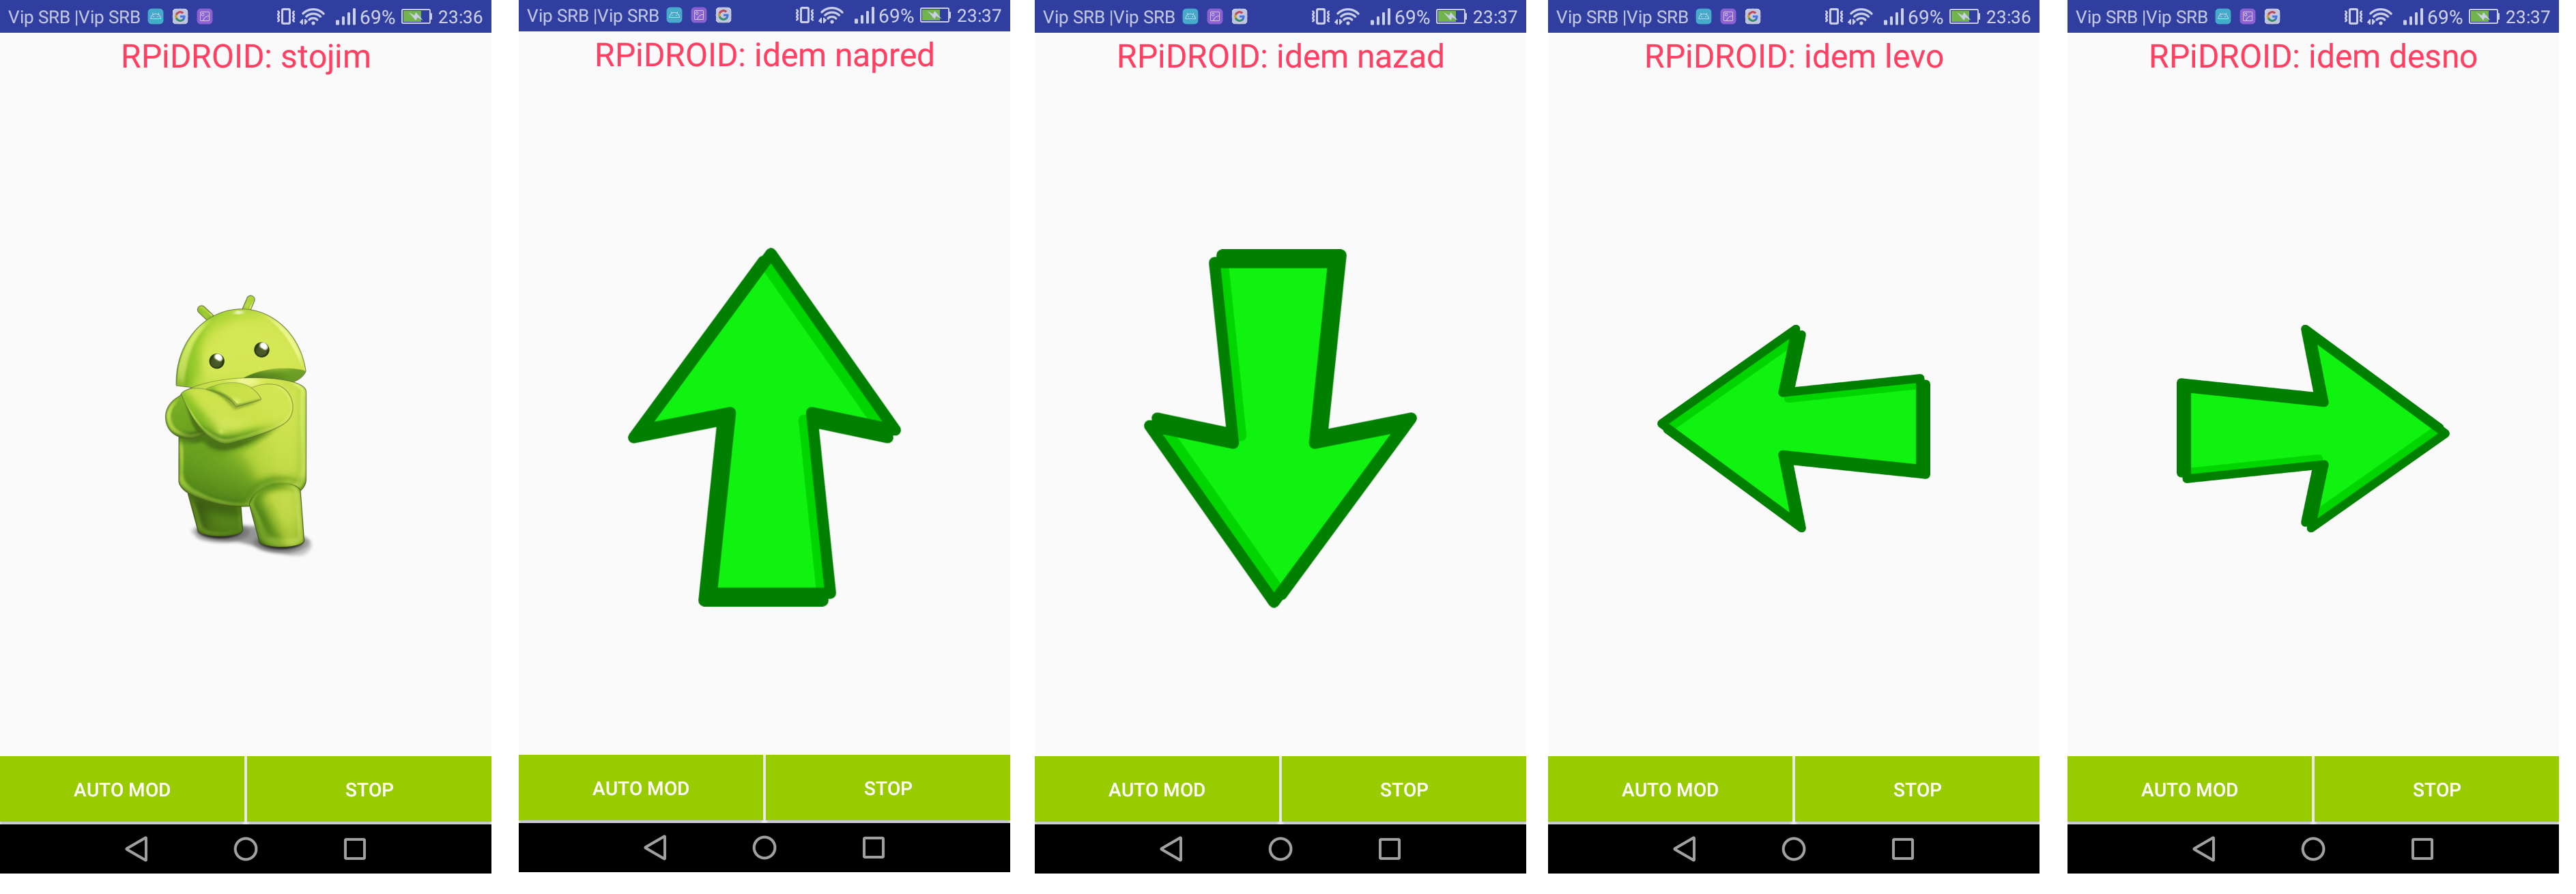
\includegraphics[width=0.9\textwidth]{slike/activity2.png}
\caption{Кориснички интерфејс активности за навођење робота}
\label{fig:uiactivity2}
\end{figure}

Ова активност такође приказује одговоре робота на корисникове команде односно на команде за навођење које му шаље апликација. Тако ће робот у одговору, уколико наиђе на препреку, јавити кориснику ту информацију и сачекати нову команду. Уколико нема препреке он ће извршити задату команду односно наставиће кретање у задатом смеру и јавити то кориснику. У зависности од одговора робота, ова активност ће променом корисничког интерфејса и доступних опција јасно ставити до знања који су дозвољени кораци које корисник може предузети. Изглед интерфејса можете видети на слици \ref{fig:uiactivity21}.

\begin{figure}[!ht]
\centering
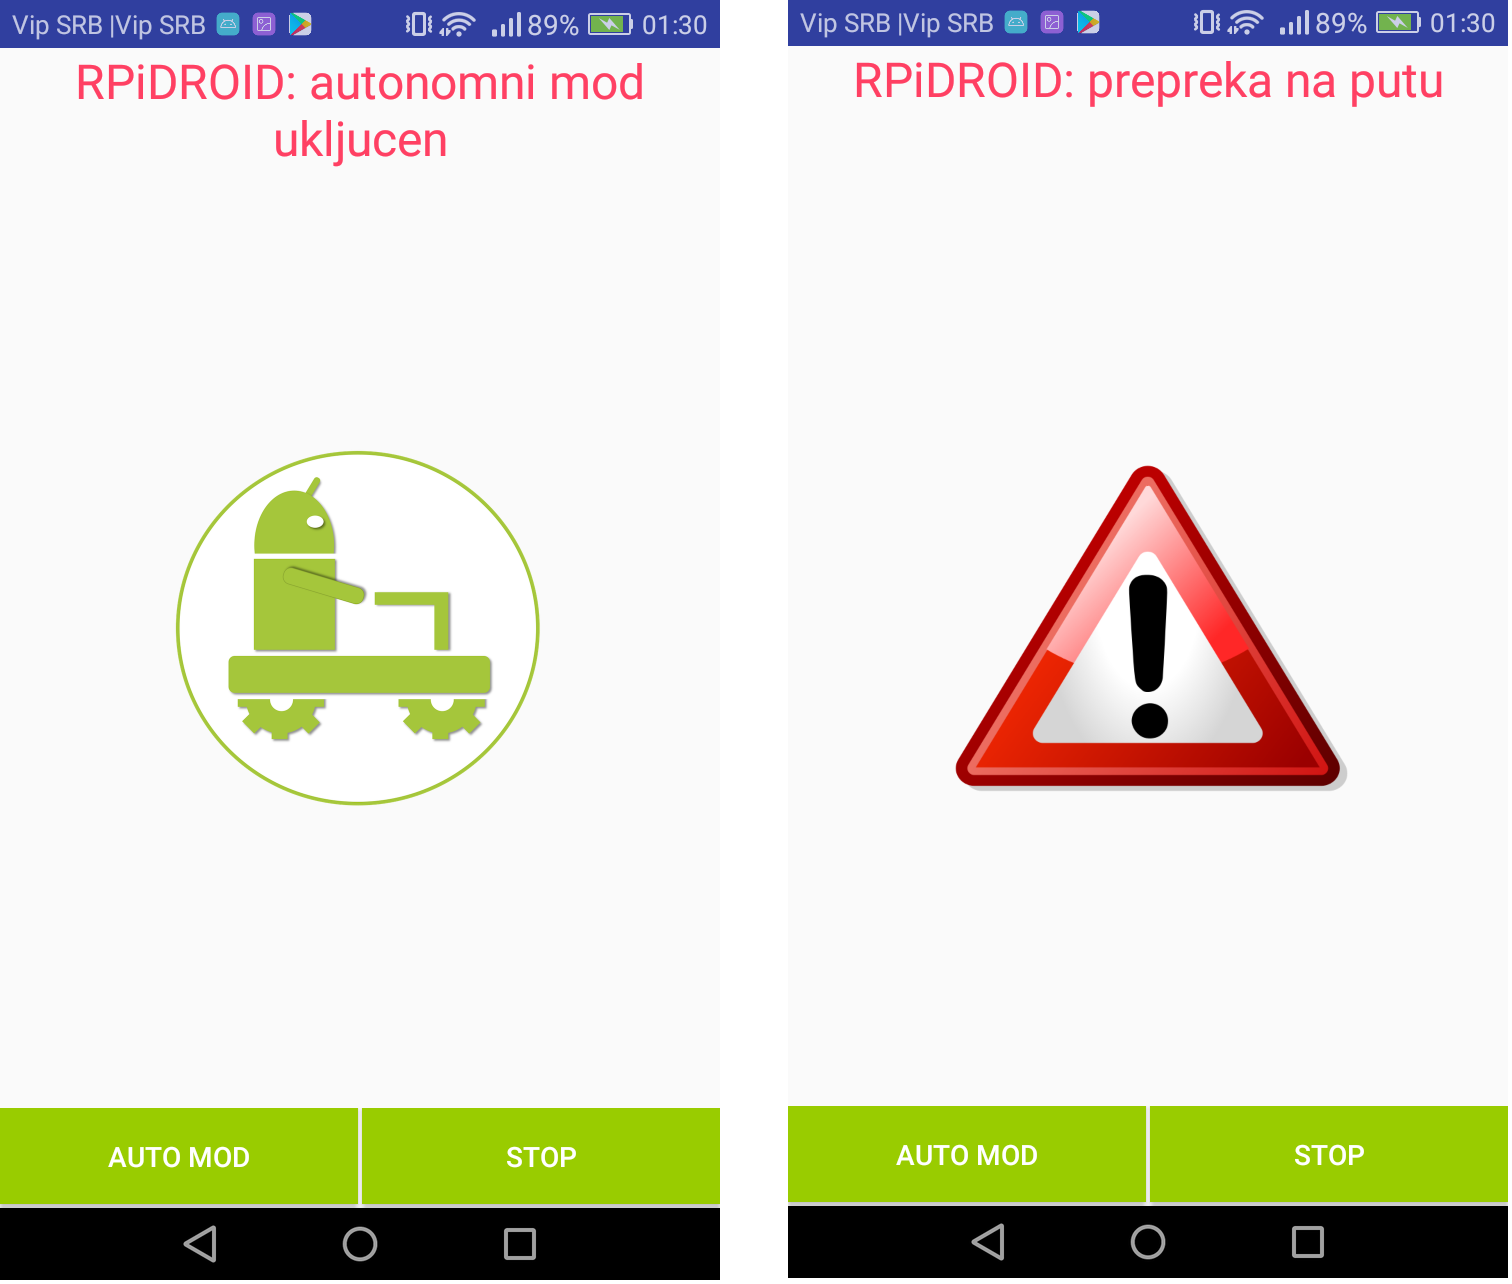
\includegraphics[width=0.4\textwidth]{slike/autoistop.png}
\caption{Обавештења робота која се приказују у апликацији}
\label{fig:uiactivity21}
\end{figure}

Поред поменутих активности апликација има и један сервис. Он апликацији омогућава комуникацију са роботом преко интернета слањем порука у складу са успостављеним протоколом комуникације. Овај сервис ради у позадини (енг.~{\em background process}) и активан је док год се апликација налази у меморији. За свако слање поруке роботу покреће нову нит (енг.~{\em thread}) из ког коришћењем HTTP протокола шаље POST захтев серверу (роботу). Слање HTTP захтева се ради из нити због тога што операције са мрежом могу трајати дуго а то може довести до кочења и рушења апликације. У телу захтева се у ЈСОН формату преносе информације релевантне за сервер. Следи један пример поруке која се шаље као команда да робот скрене у десно и добијеног одговора за успешно извршену команду:


\begin{lstlisting}[caption={Пример захтева који се шаље роботу за скретање у десно},captionpos=b]
{
  "message_type": "RPi_MSG_DIRECTION",
  "value": "GO_RIGHT"
}
\end{lstlisting}

\begin{lstlisting}[caption={Пример одговора који се добија од робота за успешно извршену команду},captionpos=b]
{
  "message_type": "RPi_MSG_DIRECTION",
  "success": "YES"
}
\end{lstlisting}

Скуп порука које апликација може послати роботу и које може добити као одговор од робота је дефинисан протоколом комуникације. Прво поље у поруци одређује тип поруке а оно одређује начин на који се интерпретира вредност из другог поља поруке (уколико оно постоји за тај тип поруке). Дозвољене вредности за тип поруке и њихово значење су:
\begin{itemize}
\item RPi\_MSG\_DIRECTION - слање команде у ком правцу да се креће робот, вредности у другом пољу означава правац кретања у односу на тренутни положај:
	\begin{itemize}
	\item 1 - напред
	\item 2 - напред полулево
	\item 3 - напред полудесно
	\item 4 - лево
	\item 5 - десно
	\item 6 - назад
	\item 7 - назад полулево
	\item 8 - назад полудесно
	\item 0 - заустави се
	\end{itemize}
\item RPi\_MSG\_CONNECTING - успостављање комуникације са роботом и његова иницијализација (прва порука у комуникацији)
\item RPi\_MSG\_DISCONNECTING - прекидање комуникације са роботом и његова деиницијализација (задња порука у комуникацији)
\item RPi\_MSG\_AUTO\_MODE - укључивање и искључивање аутономног режима кретања
	\begin{itemize}
	\item 0 - укључи аутономни режим кретања
	\item 1 - искључи аутономни режим кретања
	\end{itemize}
\item RPi\_MSG\_RESPONSE\_OK - одговор од робота, команда извршена успешно
\item RPi\_MSG\_RESPONSE\_FAILURE - одговор од робота, команда није извршена успешно
\item RPi\_MSG\_RESPONSE\_OBSTRACLE - одговор од робота, наишао на препреку
\item RPi\_MSG\_UNDEFINED - грешка у комуникацији
\end{itemize}

На слици \ref{fig:dijagramklasaapp} приказан је дијаграм класа апликације. Овај дијаграм приказује структуру апликације и интеракције међу компонентама апликације.

\begin{figure}[!ht]
\centering
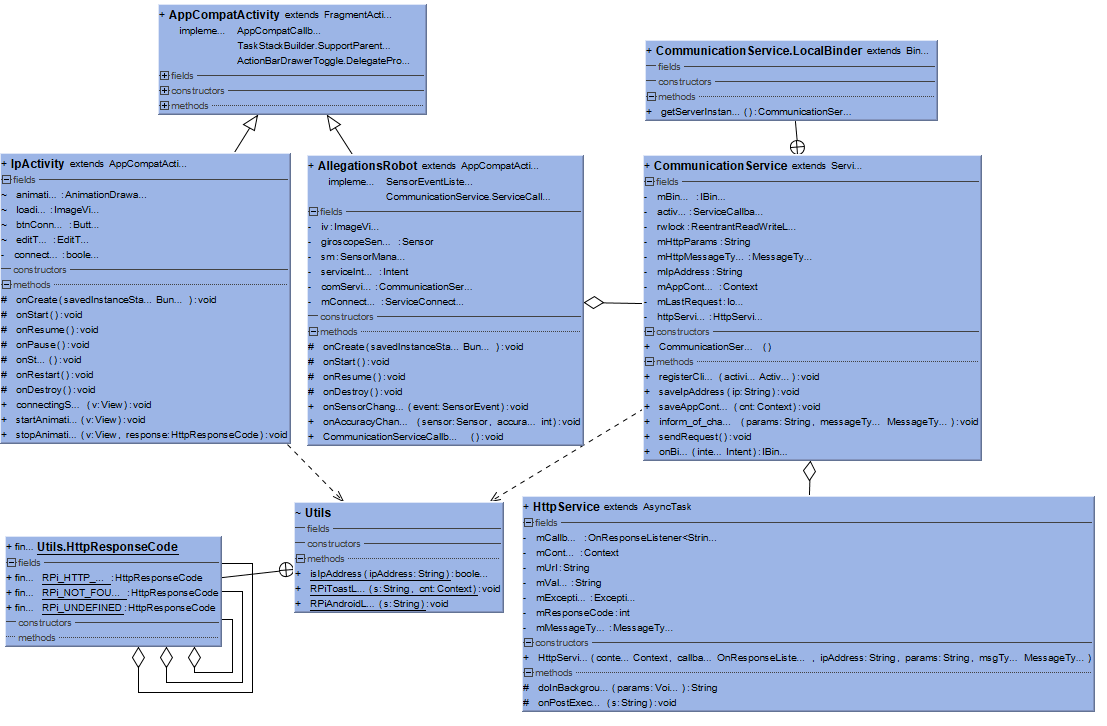
\includegraphics[width=0.9\textwidth]{slike/dijagramklasa.png}
\caption{Дијаграм класа Андроид апликације}
\label{fig:dijagramklasaapp}
\end{figure}

% ------------------------------------------------------------------------------
\section{Имплементација Пајтон апликације на Разберију}
% ------------------------------------------------------------------------------
Софтвер који се извршава на Разберију и који је намењен контроли платформе робота се може посматрати као апликација која се састоји из три модула са јасно подељеним одговорностима. Ови модули међусобно комуницирају преко АПИ-а која сваки модул нуди осталим модулима. Сликовит приказ модула и њихове међусобне комуникације можете видети на слици \ref{fig:rpisoftvare}.
Следи детаљнији опис сваког модула појединачно.
\begin{figure}[!ht]
\centering
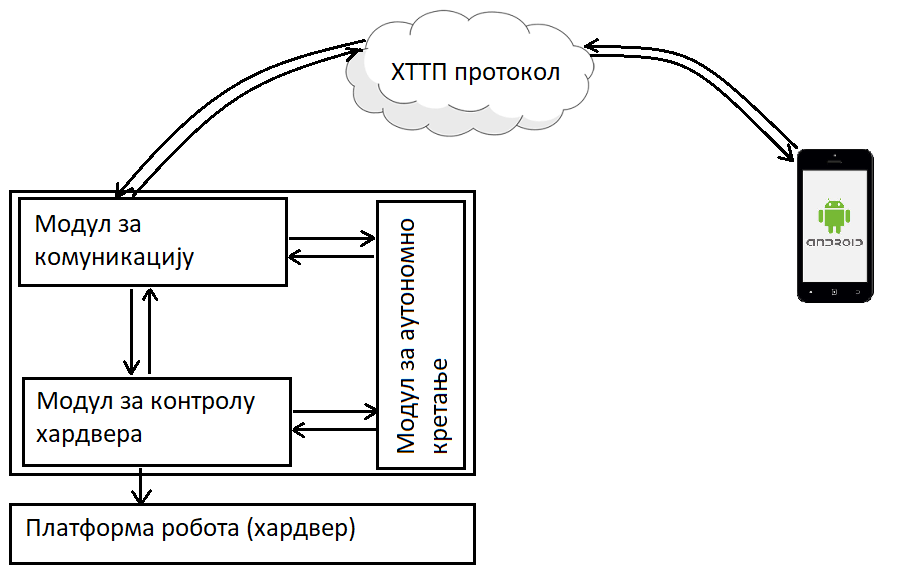
\includegraphics[width=0.7\textwidth]{slike/rpisoftvers.png}
\caption{Сликовит приказ модула апликације на Разберију и њихове сарадње}
\label{fig:rpisoftvare}
\end{figure}

\subsection{Модул за комуникацију}
Модул за комуникацију се први покреће и он мора бити активан од момента укључивања до момента искључивања робота. Овај модул се покреће чим се Разбери бутује. То се постиже тако што се у фајл 
\begin{lstlisting}
/etc/rc.local
sudo python3 /home/pi/rpidroid_robot/communication_module.py
\end{lstlisting}
дода наредба за покретање модула за комуникацију.

Модул за комуникацију је имплементиран као flask сервер. Flask је лагани  (енг.~{\em light\-weight }) веб фрејмворк написан у Пајтону. Не захтева посебне алате и библиотеке па је због тога јако погодан за уређаје са мањом количином рачунарске снаге. Нема функционалности попут слоја апстракције базе података, валидацију формата и многе друге функционалности које се обично очекују од веб сервера али упркос томе flask се може лако проширити додавањем екстензија и прилагодити сопственим потребама.
У мастер раду је дефинисана функција FlaskApplication која инстанцира објекат класе flask и она се покреће у посебној нити.  У њој се врши:
\begin{itemize}
\item Подешавање рута
\item Парсирање тела захтева 
\item Aжурирање контекста односно стања робота
\item Позивање функција из АПИ-а модула за контролу хардвера
\item Покретање модула за контролу аутономног кретања робота
\item Слање одговора и обавештења Андроид апликацији
\end{itemize}

\subsection{Модул за контролу платформе робота}
Модул за контролу платформе робота се покреће када модул за комуникацију добије захтев за повезивање са роботом од Андроид апликације, односно корисника. 
У мастер раду је имплементиран кроз функцију ControlGPIO и покреће се у посебној нити. На почетку се врши неопходна иницијализација стања свих хардверских компоненти. Комуникација са модулом за комуникацију се одвија преко објекта ContextRPi  класе Context која садржи информације о тренутном стању робота и новим командама које су стигле. Овде се такође уписују и одговори које треба вратити кориснику. Читање и ажурирање информација се штити мутексима.
Овај модул има неколико задатка:
\begin{itemize}
\item Очитавање наредне команде од модула за комуникацију кроз објекат ContextRPi
\item Покретање и заустављање мотора
\item Очитавање дистанце са сензора
\item Ажурирање стања робота кроз објекат ContextRPi
\end{itemize}

Контрола се врши кроз контролу GPIO пинова на Разберију. За контролу пинова потребно је импортовати GPIO библиотеку која долази са Разбијан оперативним системом.
\begin{lstlisting}
import RPi.GPIO as GPIO
\end{lstlisting}
Ова библиотека пружа удобан АПИ како за слање излаза тако и за очитавање улаза са GPIO пинова. У наставку је команда којом се укључује мотор који покреће леви точак робота.
\begin{lstlisting}
GPIO.output(21,GPIO.HIGH)
\end{lstlisting}

Овом командом се поставља логичка јединица на пин 21 која ће контролеру мотора пренети ту информацију а он ће провести струју до мотора и мотор ће се покренути.
За контролу мотора су коришћени пинови 2, 3, 4, 16, 20 и 21. Прва три су коришћена за десни точак а друга три за леви. Пинови 4 и 21 служе за укључивање и искључивање мотора а пинови 2 и 3 односно  16 и 20 служе да одреде смер у ком се мотор, односно точак окреће. Тако, на пример, ако се пинови поставе на следећи начин, робот ће се кретати напред.
\begin{lstlisting}
GPIO.output(16,GPIO.HIGH)
GPIO.output(20,GPIO.LOW)
GPIO.output(2,GPIO.HIGH)
GPIO.output(3,GPIO.LOW)
GPIO.output(4,GPIO.HIGH)
GPIO.output(21,GPIO.HIGH)
\end{lstlisting}

Aко би заменили вредности за пинове 16 и 20 односно 2 и 3 робот би се кретао назад. Ово је заиста лак начин за контролу али у пракси ово не ради како бисмо очекивали. Проблем је у томе што хардверске компоненте као што су ДЦ мотори немају идеално исте карактеристе па се у случају из претходног примера, уместо очекиваног понашања праволинијског кретања напред, дешава да робот благо скреће у лево или у десно. Разлог за то је мала разлика у брзини обратаја мотора која се манифестује оваквим понашањем. Решење за овај проблем је додавање радног такта за сваки од мотора. Под радним тактом се мисли на то да мотор није константно укључен већ да је део времена укључен а део времена искључен што ће се одразити на брзину обртаја точка. На овај начин се експерименталним мерењима долази до вредности тих малих пауза у раду мотора којима се поправљају разлике у самим моторима.

Још један битан задатак овог модула је очитавање вредности са сензора удаљености. Овај задатак се периодично понавља у једнаким временским интервалима. 
Овај сензор емитује ултразвучни импулс када му се сигнализира да то треба да уради и поставља логичку јединицу на свој излазни пин који је повезан са Разберијевим GPIO пином. Дистанцу до најближе препреке меримо тако што помножимо брзину простирања ултразвучних таласа са временом путовања таласа. Време се мери од момента емитовања сигнала до момента пријема одбијених сигнала од препреке. Брзина простирања ултразвучних таласа је позната и познато је време које је потребно поделити са два, јер је то време за које сигнал стигне до препреке и врати се до робота.

За окидање слања сигнала са сензора и пријем повратне информације, за један од сензора, коришћени су пинови 7 и 11. Очитавање се врши на следећи начин:
\begin{lstlisting}
PIN_TRIGGER = 7
PIN_ECHO = 11

GPIO.setup(PIN_TRIGGER, GPIO.OUT)
GPIO.setup(PIN_ECHO, GPIO.IN)

GPIO.output(PIN_TRIGGER, GPIO.LOW)

print "Racunanje razdaljine"
GPIO.output(PIN_TRIGGER, GPIO.HIGH)  #signalizacija senzoru da emituje signal
time.sleep(0.00001)
GPIO.output(PIN_TRIGGER, GPIO.LOW)

while GPIO.input(PIN_ECHO)==0:
            pulse_start_time = time.time() #vreme slanja signala
while GPIO.input(PIN_ECHO)==1:
            pulse_end_time = time.time() #vreme dobijanja odbijenog signala

pulse_duration = pulse_end_time - pulse_start_time  #razlike vremena

distance = round(pulse_duration * 17150, 2) #racunanje distrance

print "Razdaljina:",distance/2,"cm"
\end{lstlisting}


\subsection{Модул за аутономно кретање}
Модул за аутономно кретање омогућава роботу аутономно кретање тако што имплементира БАГ алгоритам описан у поглављу 4.

Када је овај режим укључен робот се креће напред све док не наиђе на препреку. Тада се тренутна позиција памти као нулта тачка и памти се тренутни правац и смер робота.\footnote{То је координатни систем који се успоставља у тренутку наиласка на препреку} 
На основу експериментално измерених вредности пређеног пута у јединици времена, у сваком кораку се ажурира позиција робота у том координатном систему и угао под којим гледа у односу на онај када је наишао на препреку. Бира страну са које ће заобићи препреку тако што провери вредности са свих сензора и анализом вредности утврди који сензори јављају отворенији пут. Након тога, у зависности од одабране стране, се репозиционира, ажурира контекст и поново покушава кретање напред, ако је могуће. Централни део имплементације се налази у следећем исечку кода:

\begin{lstlisting}
flagGo=False
obstracleDetected=False

while(True):
	targetReached=checkTarget() #proverava da li je cilj dostignut
	if(targetReached==True):	#ako jeste prekida algoritam
		break

	obstracleDetected=goAhead()	#Pokusava kretnju napred ako je moguca

	while(!obstracleDetected): #ide napred sve dok moze
		flagGo=True
		obstracleDetected=goAhead()

	side=chooseTheSide(flagGo) #kada je naisao na prepreku proverava sve senzore i bira stranu

	if(side==left):
		flagGo=False
		turnLeft5Degrees() #pravi zaokret u levo 
	else if(side==right):
		flagGo=False
		turnRight5Degrees() #pravi zaokret u desno
	
	updateContext() #azurira informacije u kontekstu
	
\end{lstlisting}

Имплементације осталих функција које се позивају се ослањају на већ описане функционалности модула за контролу хардвера са додатком математичких прорачуна. Целокупан код апликације се налази на ГитХуб-у на адреси \url{https://github.com/nenadlazic/RPiRobot.git}.


Слика \ref{fig:dijagramklasaapp} приказује дијаграм случајева употребе.

\begin{figure}[!ht]
\centering
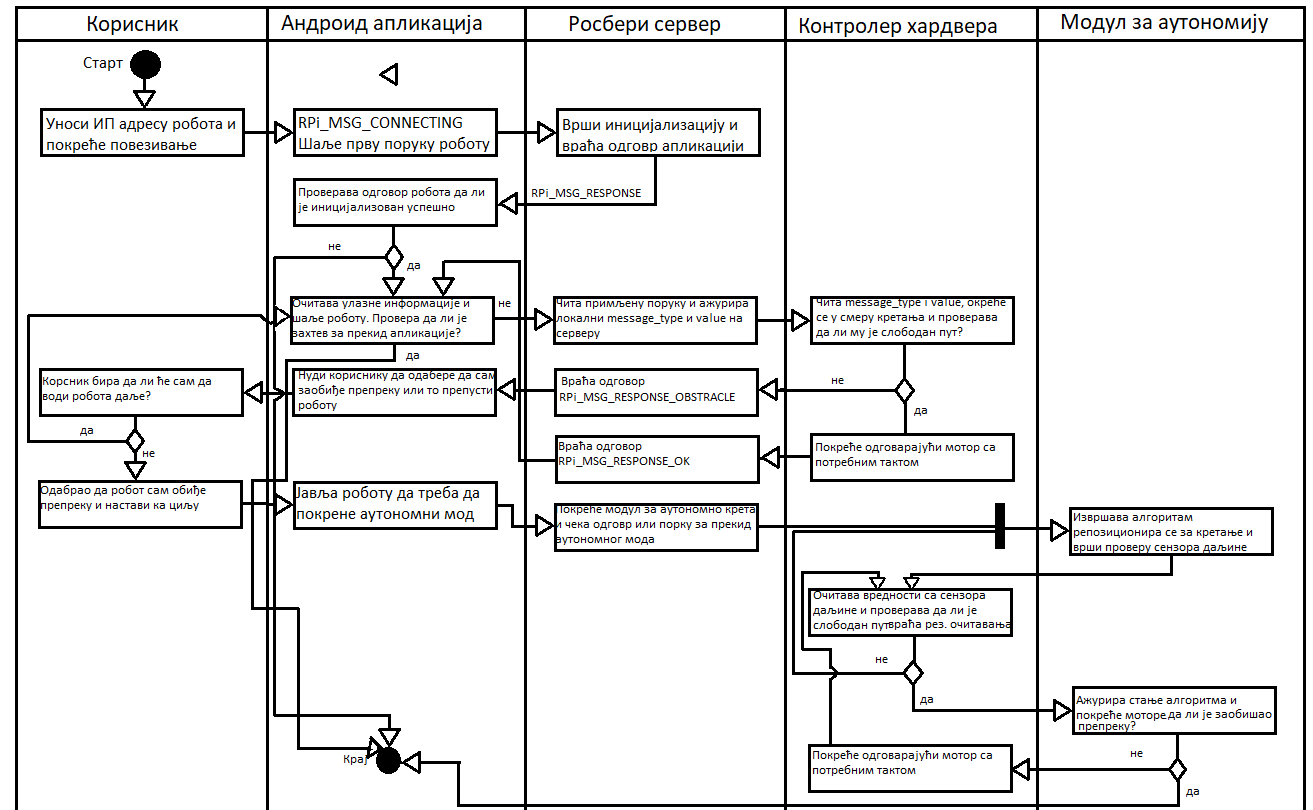
\includegraphics[width=1.0\textwidth]{slike/aktvivnostidijagram.png}
\caption{Дијаграм случајева употребе }
\label{fig:dijagramklasaapp}
\end{figure}



% ------------------------------------------------------------------------------
\chapter{Закључак}
\label{chp:zakljucak}
% ------------------------------------------------------------------------------
На самом краjу друге децениjе 21. века сведоци смо све веће присутности роботике и аутоматизациjе. Њена присутност и утицаj у будућности ће бити све већи и у све ширем спектру примена. 

У овом раду детаљно jе приказан развоj мобилног робота, корак по корак. Финални изглед робота може се видети на слици \ref{fig:finalrobot}. Количина коришћених софтверских алата и хардверских компоненти говори о томе да jе развоj jедног робота комплексан процес. Направљени робот jе потпуно функционалан. Робот се у сваком моменту може контролисати Андроид апликациjом ручним навођењем, укључивањем и искључивањем аутономног режима, а омогућено је и добијање повратних информациjа од робота. Робот има функционалну детекциjу препреке на путу, заустављање и jављање апликациjи. Алгоритам за аутономно кретање jе такође имплементиран и функционалан. Алгоритам ради са прихватљивом прецизношћу али са нешто мањом од очекиване због ограничене количине информациjа о простору и изгледу препреке коjа се може добити са коришћеним сензорима.

Развојем Андроид апликациjе за навођење потврђено је да у оквиру Андроида постоје уграђене библиотеке које имају подршку за најбитније функционалности у овом контексту као и добро документован АПИ. Писање софтвера за Разбијан у програмском jезику Паjтон се такође испоставило веома удобно, делом захваљуjући већ развиjеним библиотекама а делом и због карактеристика самог jезика Паjтон. Обе платформе, Андроид и Разбијан, су jако захвалне за рад и у потпуности су испуниле очекивања.

Сам робот има неколико места за надоградњу. Један од могућих праваца даљег рада је имплементација напреднијих алгоритама за аутономно заобилажење препрека као што је тангентни алгоритам БАГ који захтева додавање прецизнијих сензора који би могли да пруже информацију о близини препрека у свих 360 степени. Још једно побољшање којим би се могао унапредити алгоритам је додавање сензора за мерење пређеног пута како би се омогућило прецизније мерење позиције робота.  

\begin{figure}[!ht]
\centering
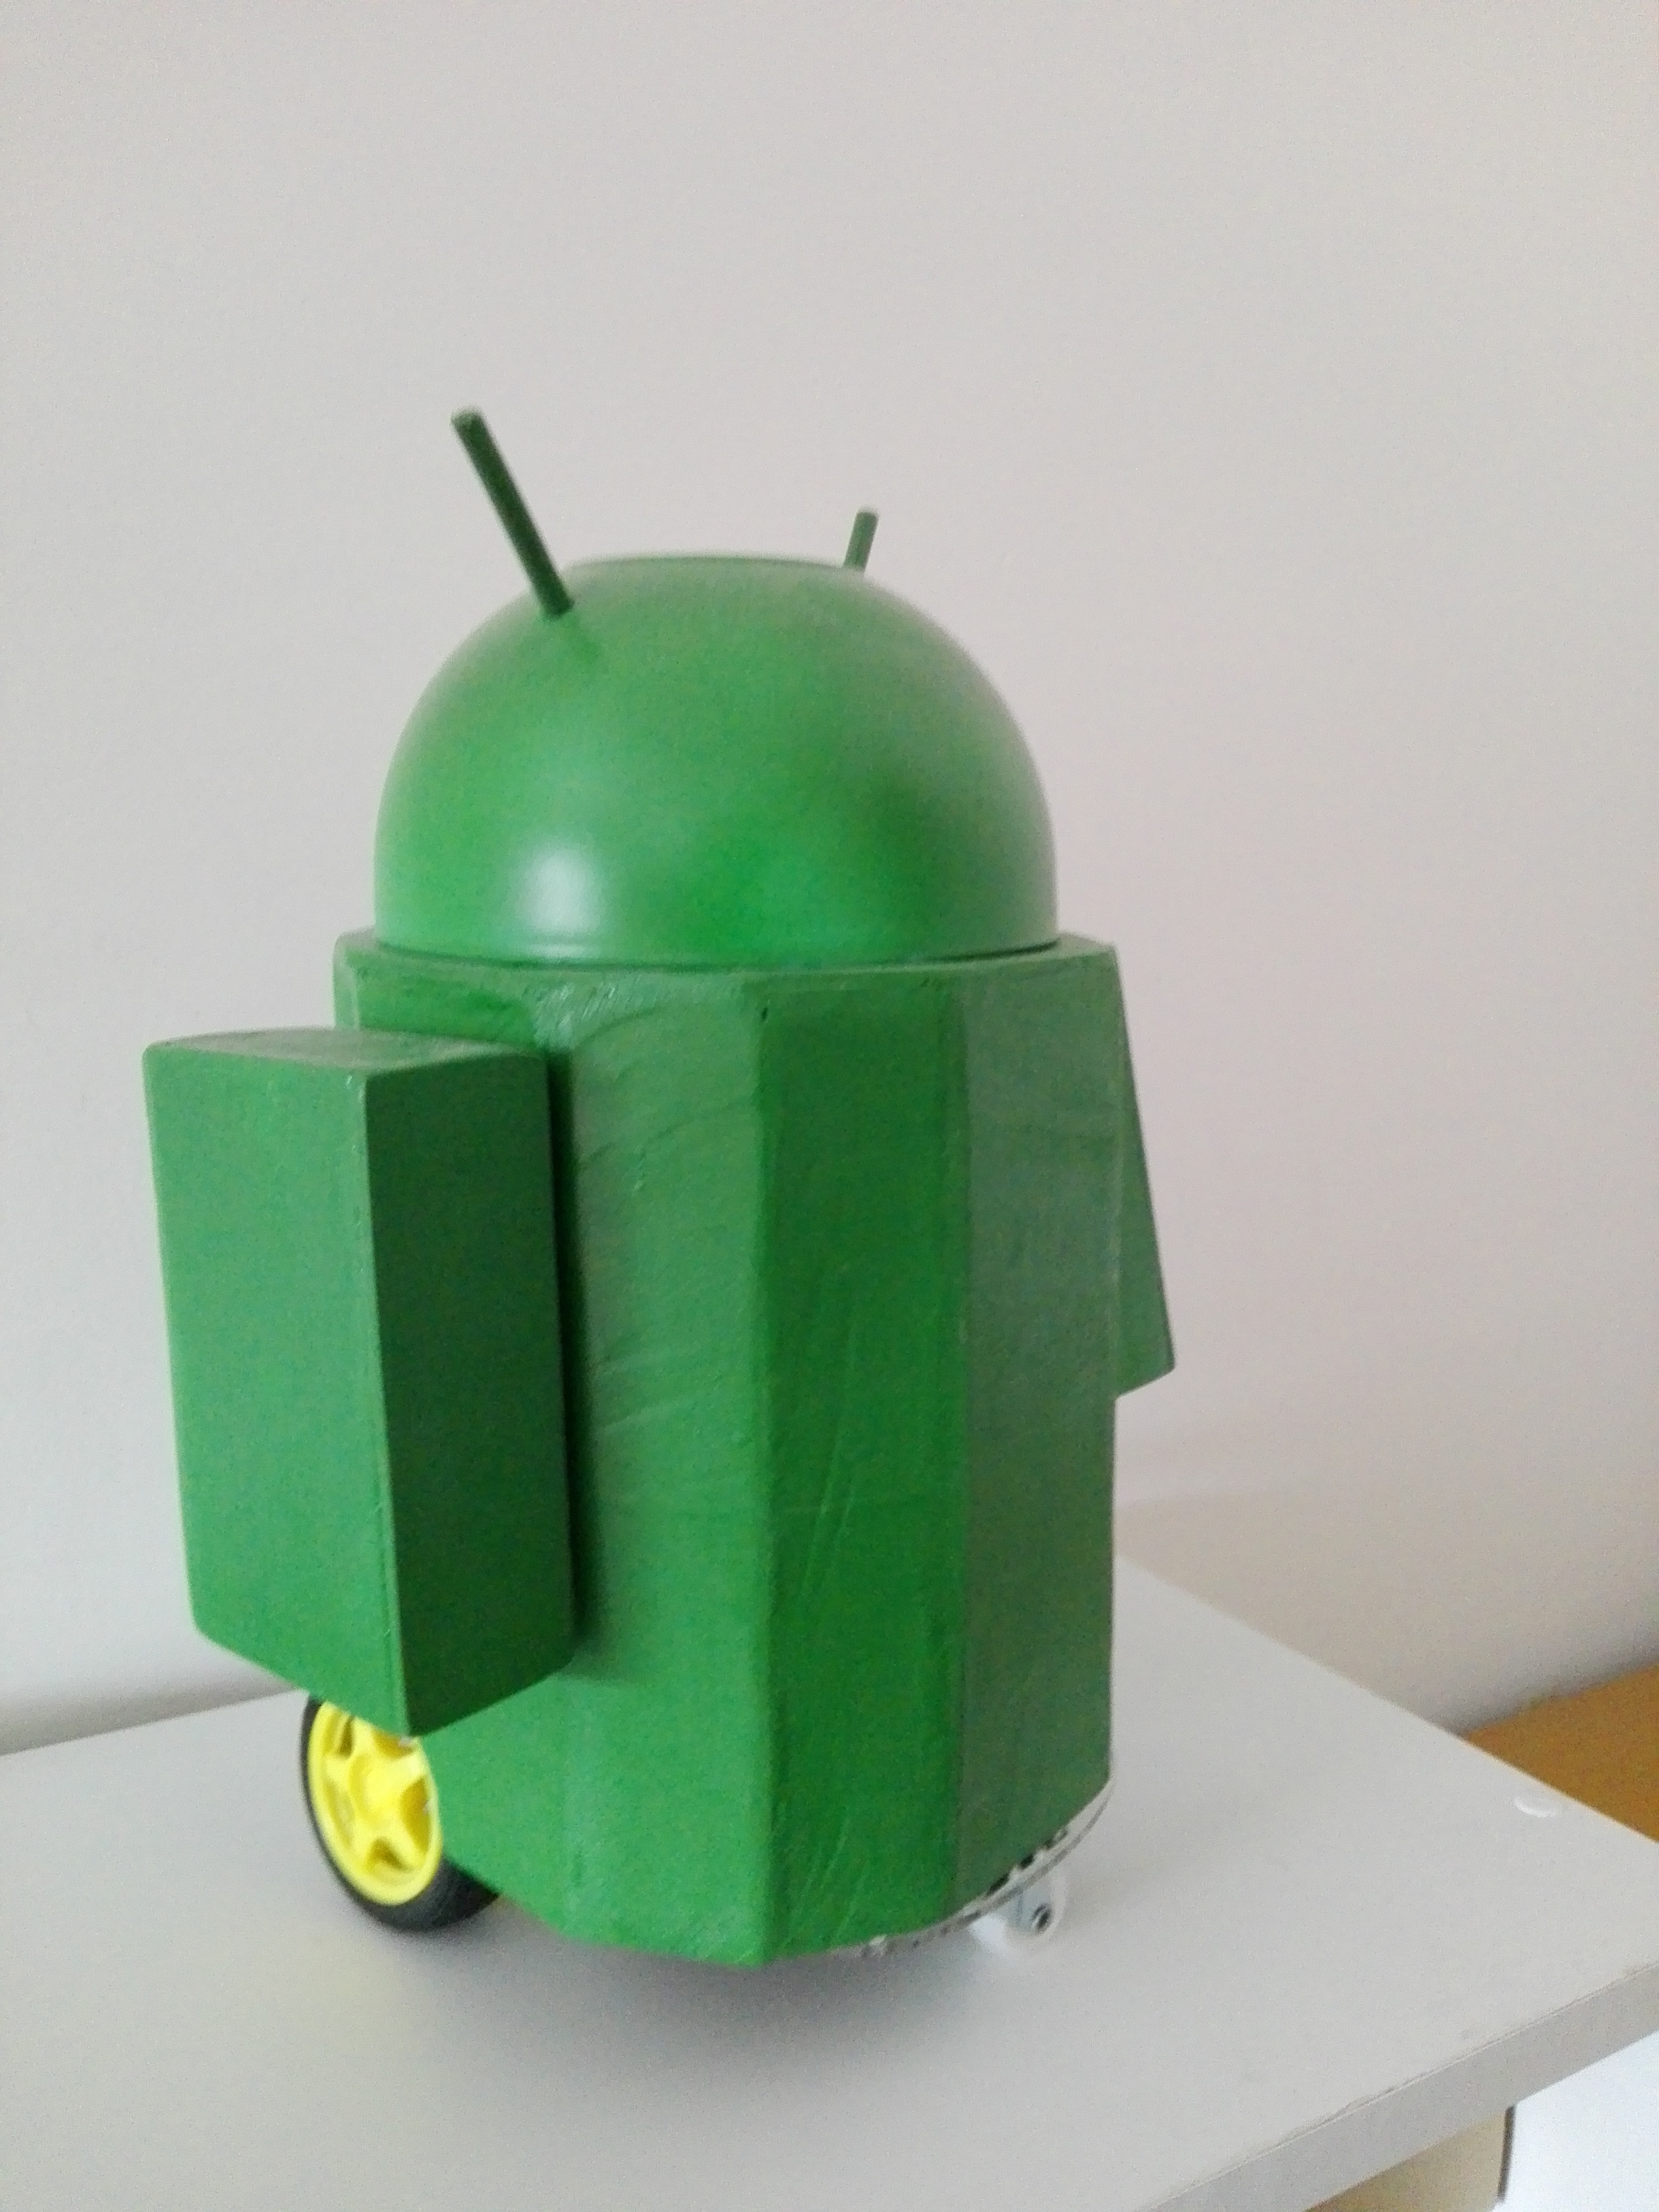
\includegraphics[width=0.80\textwidth]{slike/final.jpg}
\caption{Изглед робота након завршетка рада и склапања}
\label{fig:finalrobot}
\end{figure}

% ------------------------------------------------------------------------------
% Literatura
% ------------------------------------------------------------------------------
\literatura




% ==============================================================================
% Završni deo teze i prilozi
\backmatter
% ==============================================================================

% ------------------------------------------------------------------------------
% Biografija kandidata
\begin{biografija}
\textbf{Ненад Лазић} 
Рођен сам у Љубовији 13. фебруара 1993. године. Основну школу Доситеј Обрадовић сам завршио у Љубовији 2008. године 
након чега сам уписао Техничку школу у Ваљеву, смер електротехничар рачунара. Током средње школе заволео сам програмирање
и математику због чега сам одлучио да мој избор у наставку школовања буде Математички факултет у Београду. На Математички факултет
сам се уписао 2012. године на смеру Информатика. Основне академске студије сам завршио 2015. године након којих сам уписао мастер студије.

\end{biografija}
% ------------------------------------------------------------------------------

\end{document} 